% Settings for the default beamer theme
\documentclass[english, aspectratio=169]{beamer}
\usepackage[T1]{fontenc}
\usepackage[utf8]{inputenc}
\usepackage{tabularx}
\usepackage{babel}
\usepackage[ruled,vlined]{algorithm2e}
\SetAlgorithmName{Algoritmus}{algoritmus}{List of Algorithms}
\setcounter{secnumdepth}{3}
\setcounter{tocdepth}{3}

\makeatletter

\newcommand\makebeamertitle{\frame{\maketitle}}

% (ERT) argument for the TOC
\AtBeginDocument{%
  \let\origtableofcontents=\tableofcontents
  \def\tableofcontents{\@ifnextchar[{\origtableofcontents}{\gobbletableofcontents}}
  \def\gobbletableofcontents#1{\origtableofcontents}
}

% Theme settings
\usetheme{Frankfurt}
\usecolortheme{default}
\usefonttheme[onlymath]{serif}

% Template settings
\setbeamertemplate{navigation symbols}{}
\setbeamertemplate{blocks}[rounded][shadow=false]
\setbeamertemplate{title page}[default][colsep=-4bp, rounded=true, shadow=false]
\makeatother

\begin{document}

% Title page
\section{Bevezetés}
\title[]{Üzleti Intelligencia}
\subtitle{8. Előadás: Objektum detekció}
\author[Kuknyó Dániel]{Kuknyó Dániel\\Budapesti Gazdasági Egyetem}
\date{2023/24\\1.félév}
\makebeamertitle

% Table of contents slide
\begin{frame}
\tableofcontents{}
\end{frame}

% Table of contents of the current section
\begin{frame}
\tableofcontents[currentsection]
\end{frame}

\begin{frame}{Osztályozás}
\begin{columns}
\begin{column}{.5\textwidth}
Osztályozás esetén a neurális hálózat output rétegében minden lehetséges osztályhoz egy neuron tartozik. A neuronok azt a valószínűséget becsülik meg, hogy \textbf{az adott mintaegyed mekkora valószínűséggel esik a neuronhoz tartozó kategóriába}.\par\smallskip
Ez a \textbf{softmax} réteg, ahol az egyes neuronok aktivációs függvénye a softmax függvény. A softmax rétegben lévő neuronok outputjainak összege mindig $1$.
\end{column}
\begin{column}{.5\textwidth}
\begin{center}
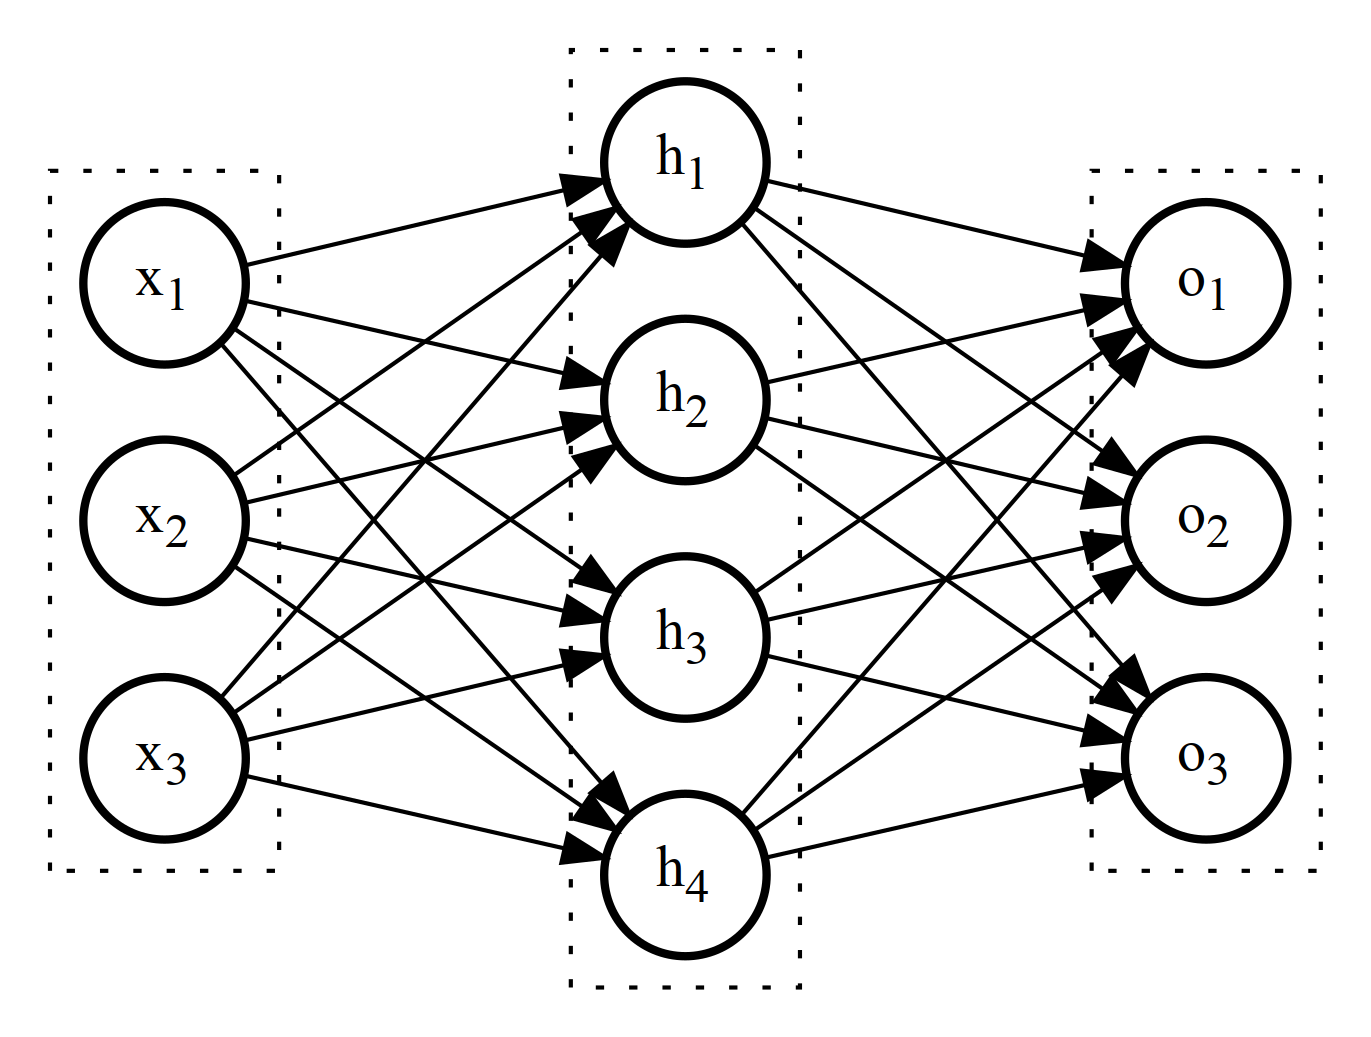
\includegraphics[width=7cm, keepaspectratio]{../../7_dl/doc/graphs/dl_1.png}
\end{center}
\end{column}
\end{columns}
\end{frame}

\begin{frame}{Predikció osztályozás esetén}
\begin{columns}
\begin{column}{.7\textwidth}
A legegyszerűbb módja az osztályozásnak, ha a hálózat outputként \textbf{összesen egy címkét} ad outputként, ami a predikciója az input képre (vagy adatra) vonatkozóan.\par\smallskip
Ebben az esetben a hálózat softmax rétege azt becsüli meg, hogy \textbf{mekkora válószínűséggel tartozik a mintaegyed a tanító osztályok valamelyikébe}. Például:
\[
\left[ macska: 0.9; kutya: 0.1 \right]
\]
Ezután az output úgy áll elő, hogy a hálózat \textbf{kiválasztja a legnagyobb valószínűségű osztályt} az $argmax$ operátorral, majd visszaadja a legnagyobb valószínűséghez tartozó címkét.
\end{column}
\begin{column}{.3\textwidth}
\begin{center}
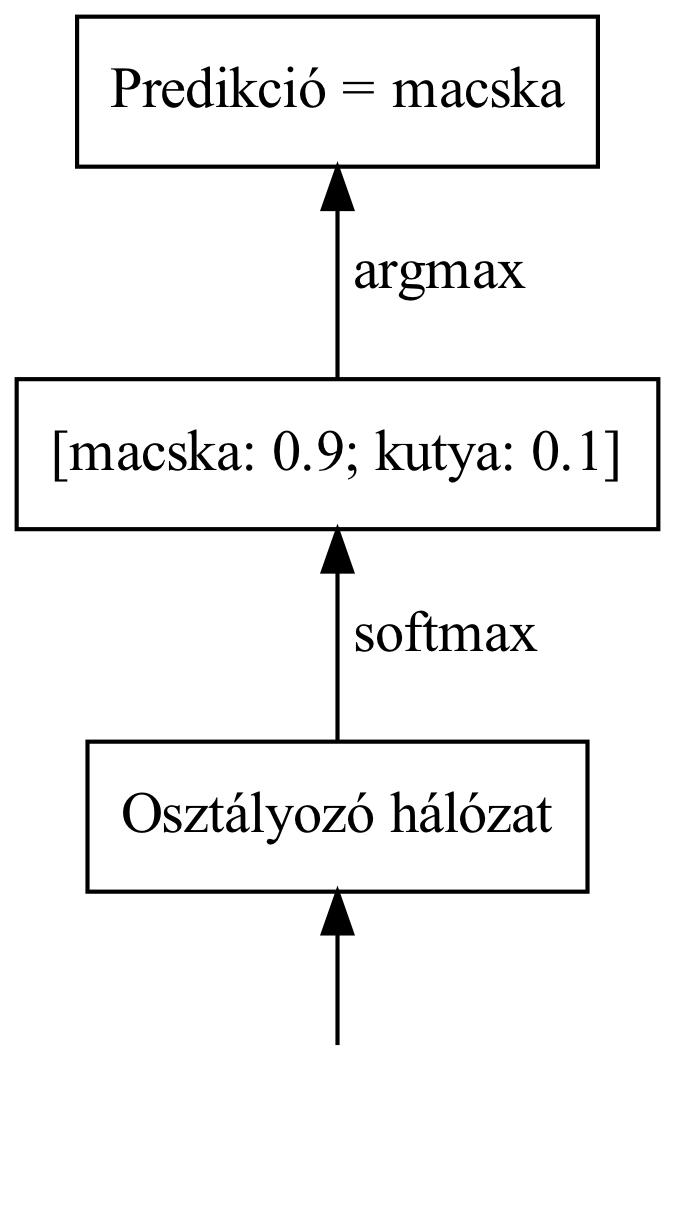
\includegraphics[height=5cm, keepaspectratio]{graphs/od_1.png}\\
\vspace{-0.7cm}
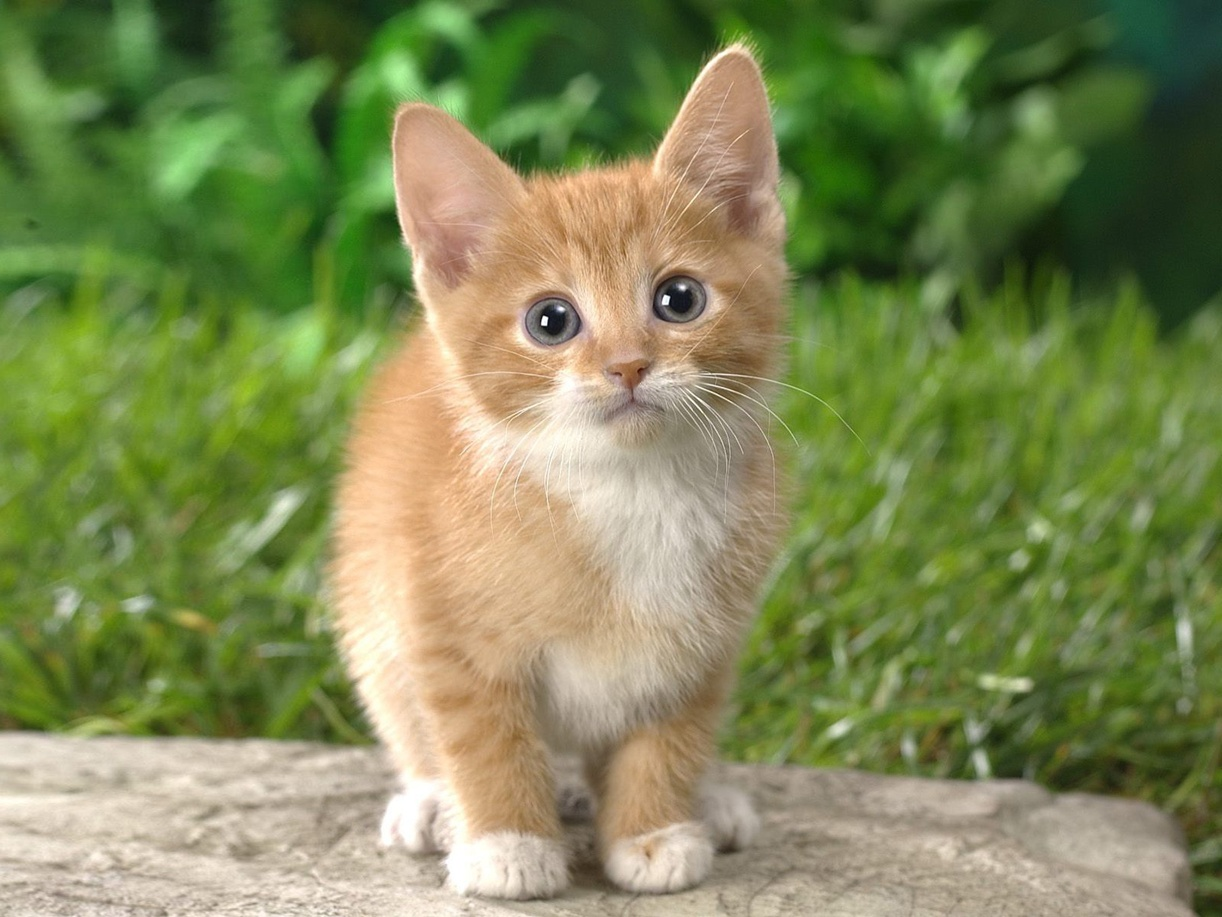
\includegraphics[height=2.5cm, width=2.5cm, keepaspectratio]{images/od_1.png}
\end{center}
\end{column}
\end{columns}
\end{frame}

\begin{frame}{Lokalizáció}
\begin{columns}
\begin{column}{.7\textwidth}
Az objektum lokalizáció feladata az osztályozás egy speciális esete. A lokalizáció problémájában nem csak azt kell megbecsülnie a neurális hálózatnak, hogy milyen objektum található egy képen, hanem meg is kell adnia az \textbf{objektum pozícióját azzal, hogy megadja a kereteződobozának koordinátáit}.\par\smallskip
Ebben az esetben a hálózat outputja nem csak egy címke, hanem a dobozt meghatározó négy koordináta is. Ezek a leggyakrabban:
\begin{itemize}
	\item $x$: A doboz bal felső sarkának $x$ koordinátája.
	\item $y$: A doboz bal felső sarkának $y$ koordinátája.
	\item $w$: A doboz szélessége (width).
	\item $h$: A doboz magassága (height).
\end{itemize}
\end{column}
\begin{column}{.3\textwidth}
\begin{center}
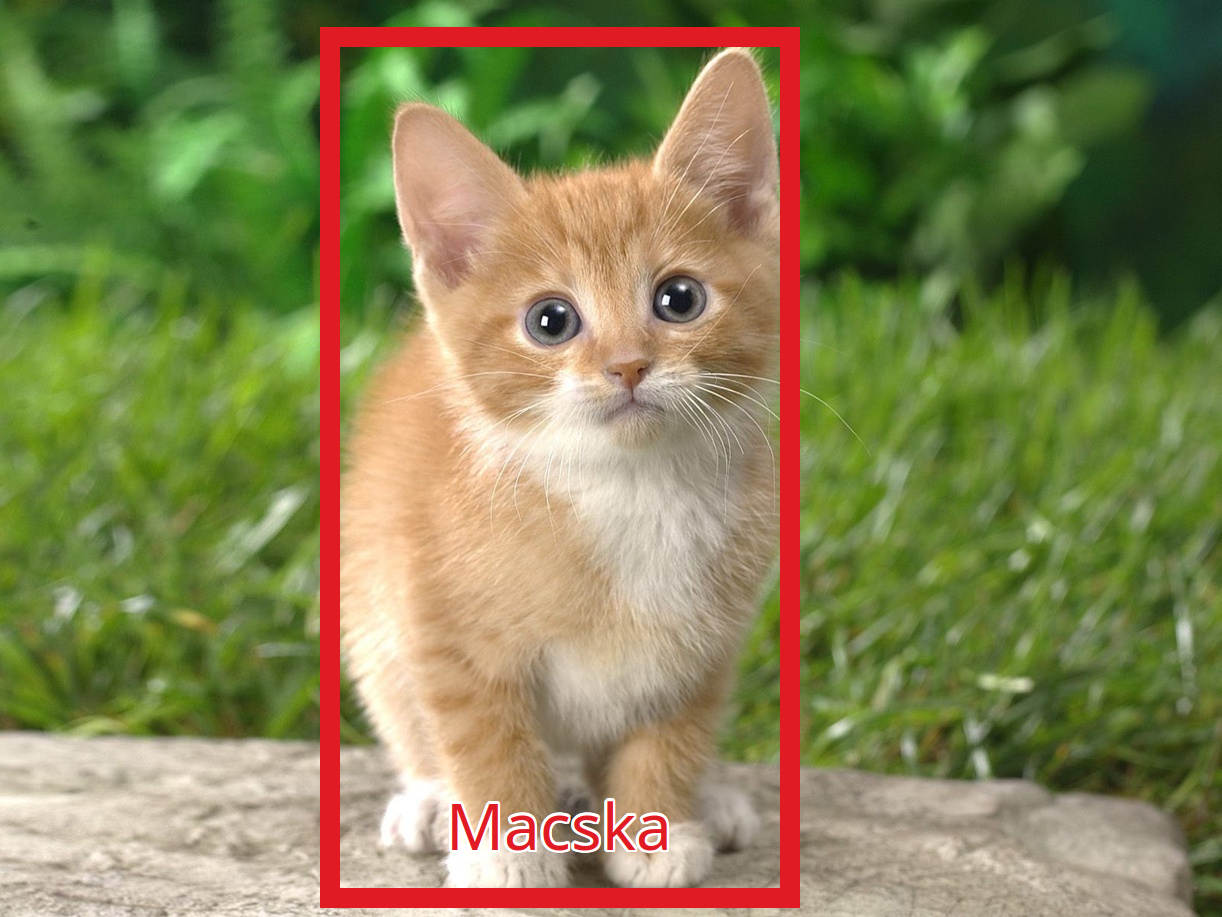
\includegraphics[width=4cm, keepaspectratio]{images/od_2.png}
\end{center}
\end{column}
\end{columns}
\end{frame}

\begin{frame}{Predikció lokalizáció esetén}
\begin{columns}
\begin{column}{.6\textwidth}
Lokalizáció esetén a neurális hálózat két részre ágazik, mivel két különböző feladatot kell elvégeznie:\par\smallskip
\textbf{Osztályozás}: ez megegyezik az osztályozó hálózat által végzett feladattal. A hálózat megbecsül egy valószínűségeloszlást, majd ebből kiválasztja a legnagyobb valószínűséghez tartozó osztályt, amit visszaad mint predikció.\par\smallskip
\textbf{Kereteződoboz predikciók}: a lokalizáció feladatához a neurális hálózatnak meg kell becsülnie az érdekelt régiók dobozainak koordinátáit. A neurális hálózat kiválasztja a becsült kereteződobozok közül azt, amelyik \textbf{a legnagyobb valószínűséggel tartalmazza a keresett objektumot}. 
\end{column}
\begin{column}{.4\textwidth}
\begin{center}
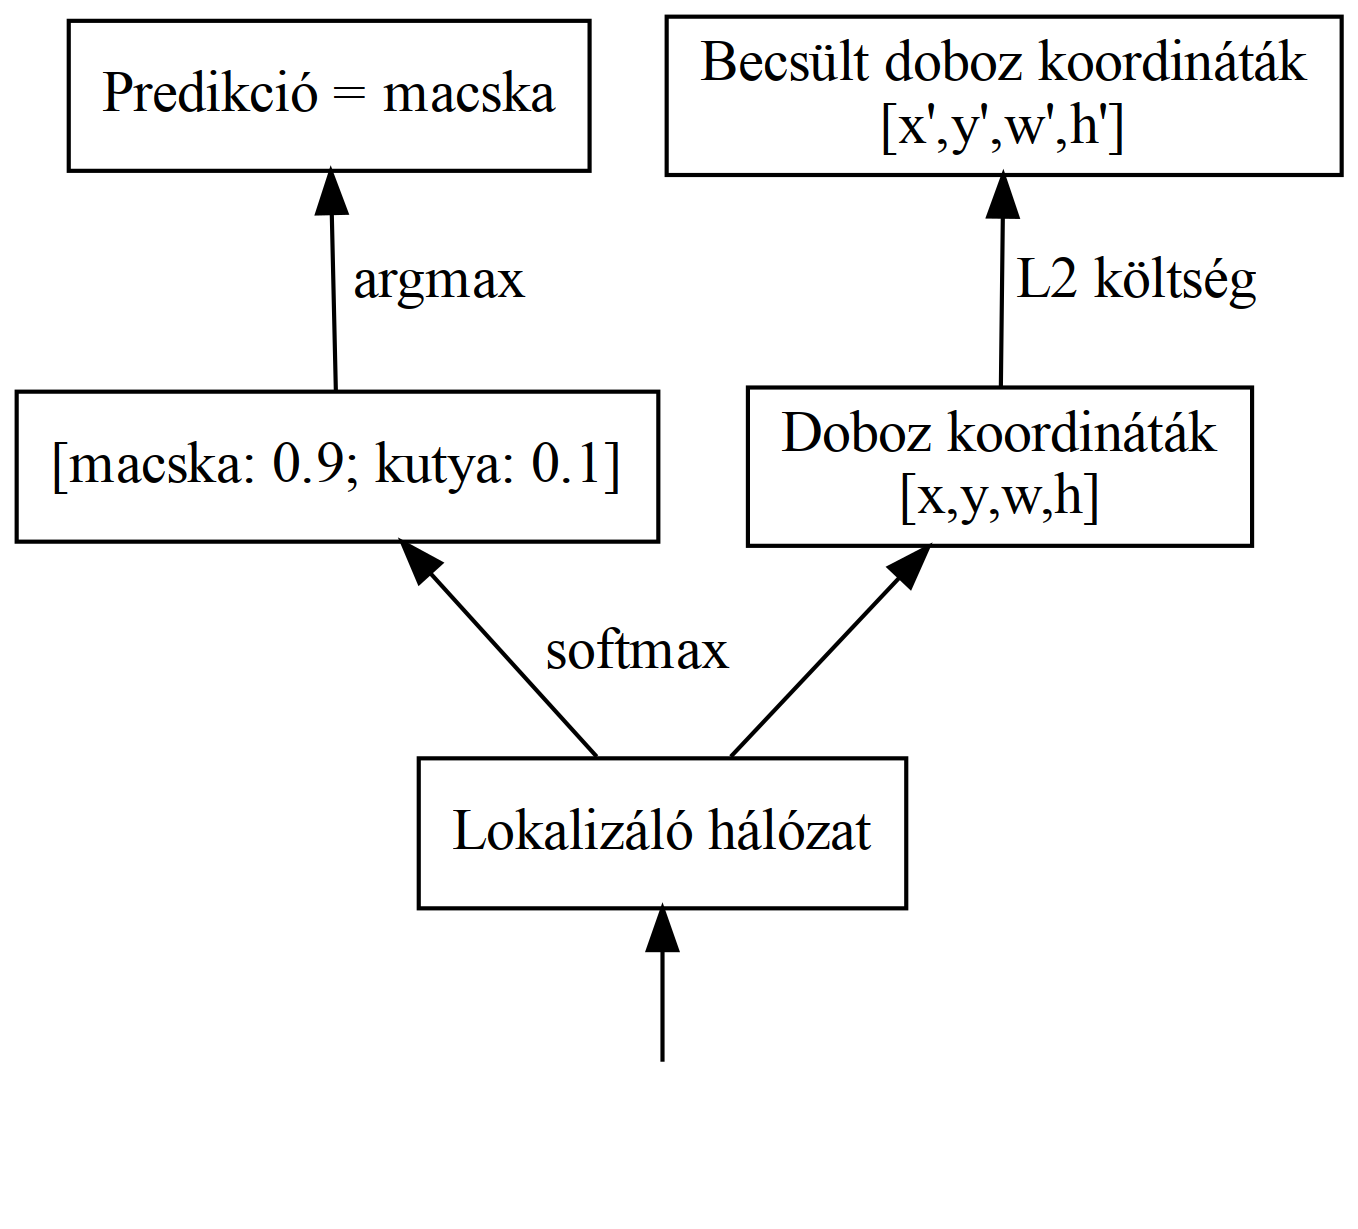
\includegraphics[height=5cm, keepaspectratio]{graphs/od_2.png}\\
\vspace{-0.7cm}
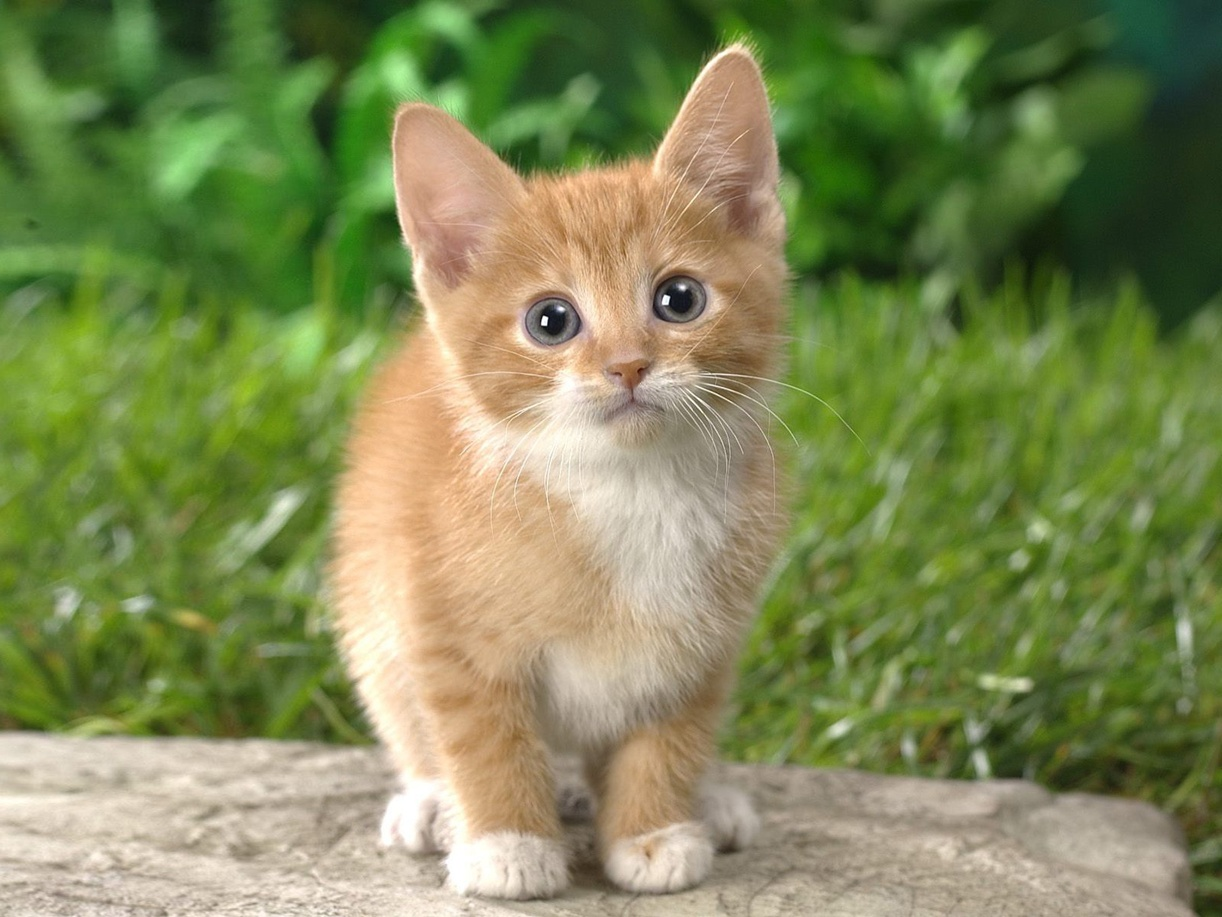
\includegraphics[height=2.5cm, width=2.5cm, keepaspectratio]{images/od_1.png}
\end{center}
\end{column}
\end{columns}
\end{frame}

\begin{frame}{Pontosság mérése kereteződobozokkal}
\begin{columns}
\begin{column}{.7\textwidth}
Mivel az objektum detekció egy felügyelt tanulási algoritmus, \textbf{szüksége van címkékre}. Ebben az esetben a címkék a valós osztályt és a kereteződoboz $x,y,w,h$ koordinátáit tartalmazzák.\par\smallskip
A jóságfüggvény $A$ valós és $B$ becsült kereteződoboz koordinátáit hasonlítja össze az IoU (metszet/unió) mérőszámmal:
\[
IoU=\frac{A \cap B}{A \cup B}
\]
Tehát minél jobban illeszkedik a becsült doboz a valósra, annál közelebb van a mérőszám $1$-hez. Ha a két doboznak nincs közös területe, $IoU=0$.
\end{column}
\begin{column}{.3\textwidth}
\begin{center}
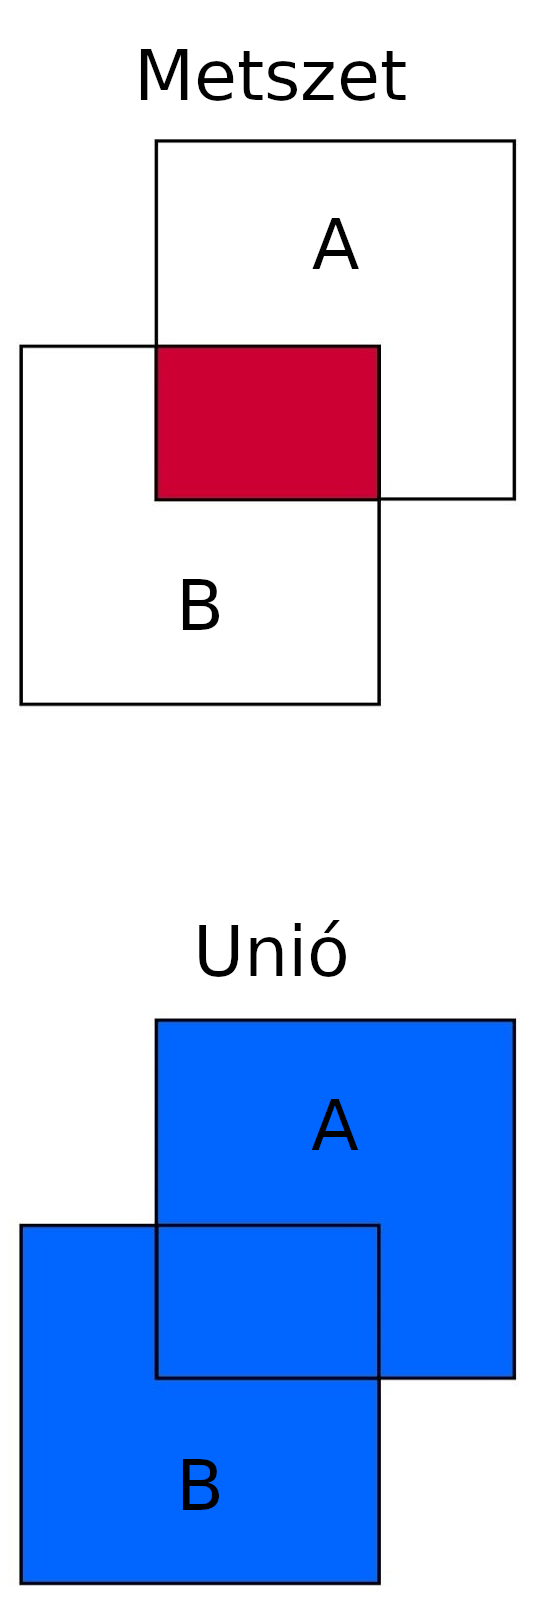
\includegraphics[height=7cm, width=7cm, keepaspectratio]{images/od_9.png}
\end{center}
\end{column}
\end{columns}
\end{frame}

\section{Objektum detekció}

\begin{frame}
\tableofcontents[currentsection]
\end{frame}

\begin{frame}{Objektum detekció}
\begin{columns}
\begin{column}{.5\textwidth}
Az objektum detekció a lokalizáció általánosítása több objektumra egyetlen képen belül. Ebben az esetben a neurális hálózat feladata \textbf{minden ismert objektum lokalizálása a képen}.\par\smallskip
Ebben az esetben a hálózat outputja minden egyes ismert objektumra: 
\begin{itemize}
	\item Az objektum becsült címkéje.
	\item Az objektum kereteződobozának $x,y,w,h$ koordinátái. 
\end{itemize}
Mivel az érdekelt objektumok száma képenként eltérő lehet, az \textbf{objektum detekciós hálózatok outputjainak számossága is képenként különbözik}!
\end{column}
\begin{column}{.5\textwidth}
\begin{center}
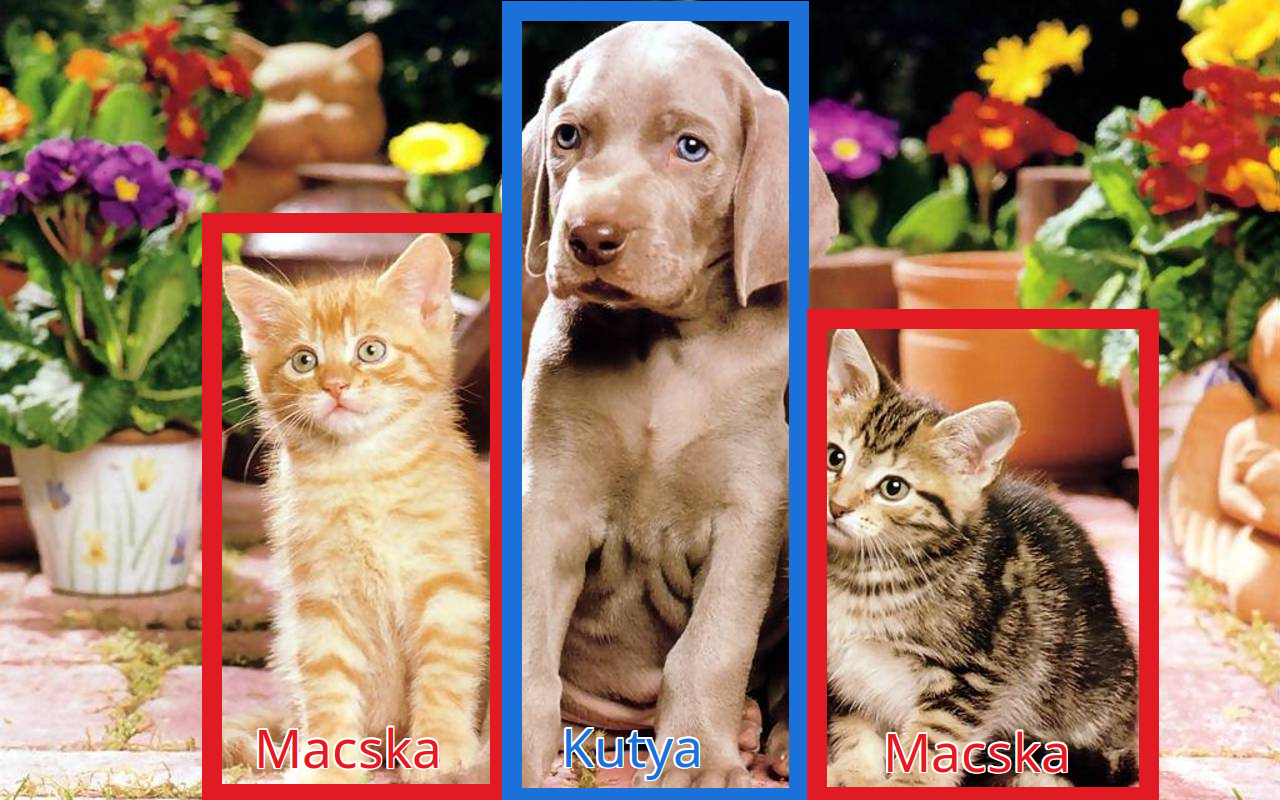
\includegraphics[width=7cm, keepaspectratio]{images/od_4.png}
\end{center}
\end{column}
\end{columns}
\end{frame}

\begin{frame}{Kezdeti detektor implementáció}
\begin{columns}
\begin{column}{.6\textwidth}
Az első objektum detektor modellek implementációi meglehetősen naívak voltak. Az eljárás szerint a modell \textbf{végigcsúsztat egy előre meghatározott méretű ablakot a képen}, és minden egyes általa meghatározott képről eldönti, \textbf{hogy háttér-e} ($bgr$) vagy valamelyik keresett osztályba tartozik-e:
\only<1>{
\[
output = [bgr: 0.8, kutya: 0.1, macska: 0.1]
\]
Ebben az esetben $\hat{y}=\underset{p}{argmax}(output)=bgr$, és az algoritmus eldobja a kereteződoboz predikcióját.
}
\only<2>{
\[
output = [bgr: 0.0, kutya: 0.01, macska: 0.99]
\]
Ebben az esetben $\hat{y}=\underset{p}{argmax}(output)=macska$, és a becsült kereteződoboz az, ahol a legnagyobb a keresett osztály valószínűsége.
}
\end{column}
\begin{column}{.5\textwidth}
\only<1>{
\begin{center}
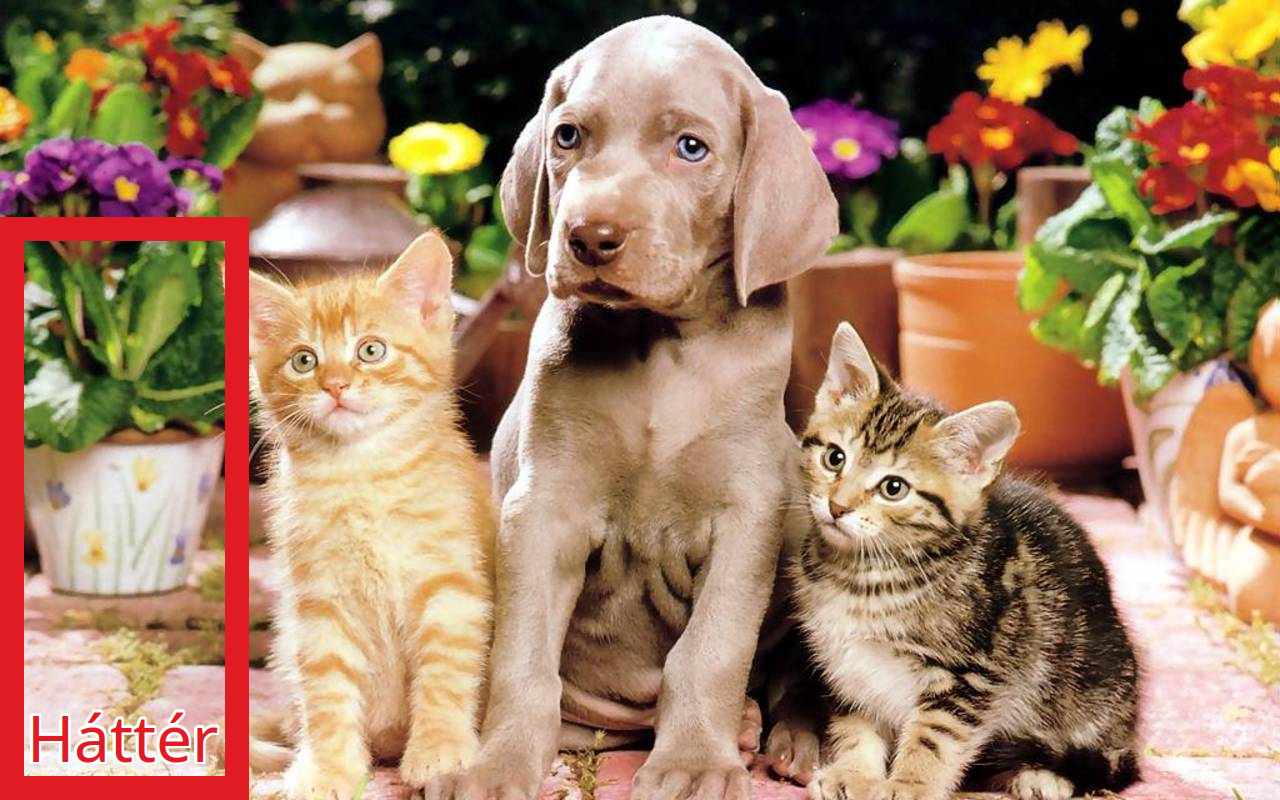
\includegraphics[width=7cm, keepaspectratio]{images/od_5.png}
\end{center}}
\only<2>{
\begin{center}
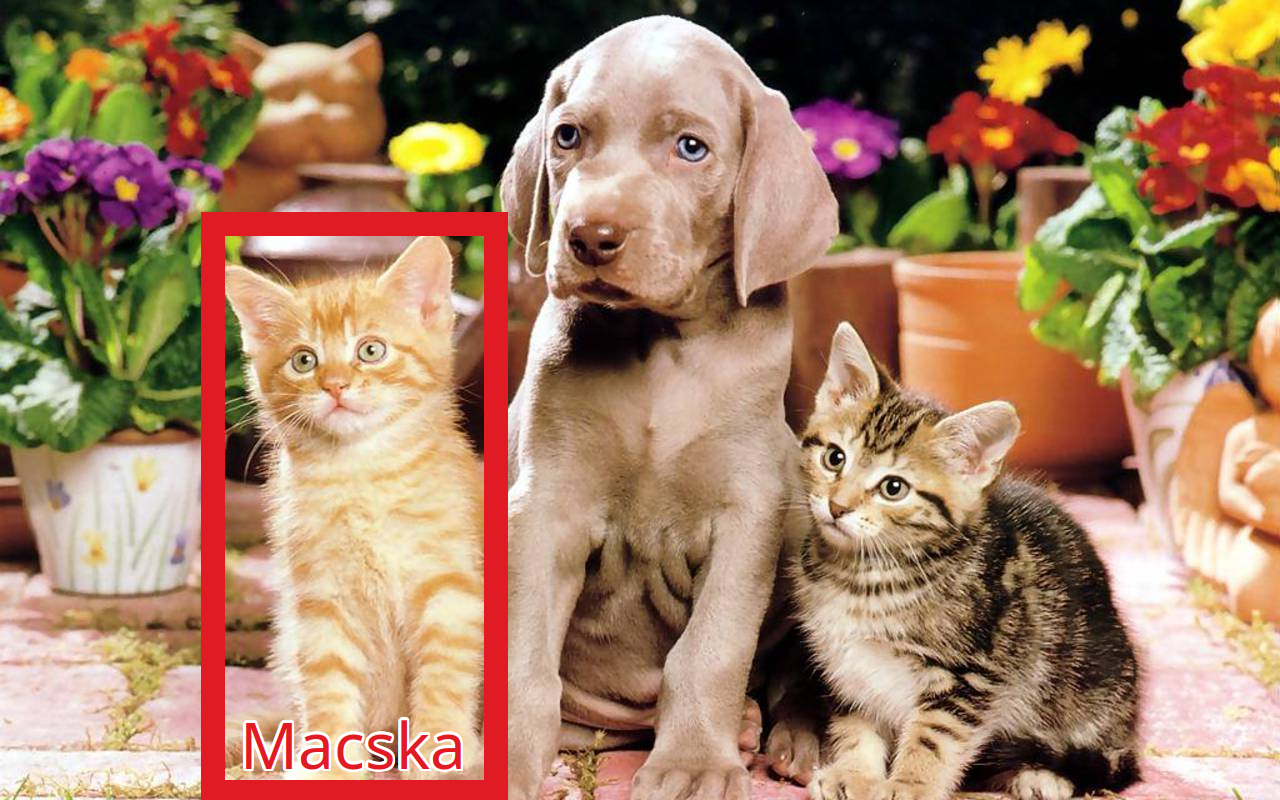
\includegraphics[width=7cm, keepaspectratio]{images/od_6.png}
\end{center}
}
\end{column}
\end{columns}
\end{frame}

\begin{frame}{Miért nem lehetséges ez az implementáció?}
\begin{columns}
\begin{column}{.7\textwidth}
Hány lehetséges kereteződoboz van egy $H \cdot W$ méretű képen?\par\medskip
Ha van egy $h \cdot w$ méretű kereteződoboz a lehetséges $x$ koordináták száma $W-w+1$, és a lehetséges $y$ koordináták száma $H-h+1$. A lehetséges megoldások száma egyetlen kereteződoboz méretre: $(W-w+1) \cdot (H-h+1)$.\par\medskip
Az összes lehetséges kereteződoboz méretre pedig:
\[
\sum_{h=1}^H \sum_{w=1}^W (W-w+1) \cdot (H-h+1) = \frac{H(H+1)}{2} \frac{W(W+1)}{2}
\]
Ez azt jelenti, hogy egy $800 \cdot 600$ méretű képre $\sim 58$ millió lehetséges kereteződoboz létezik.
\end{column}
\begin{column}{.3\textwidth}
\begin{center}
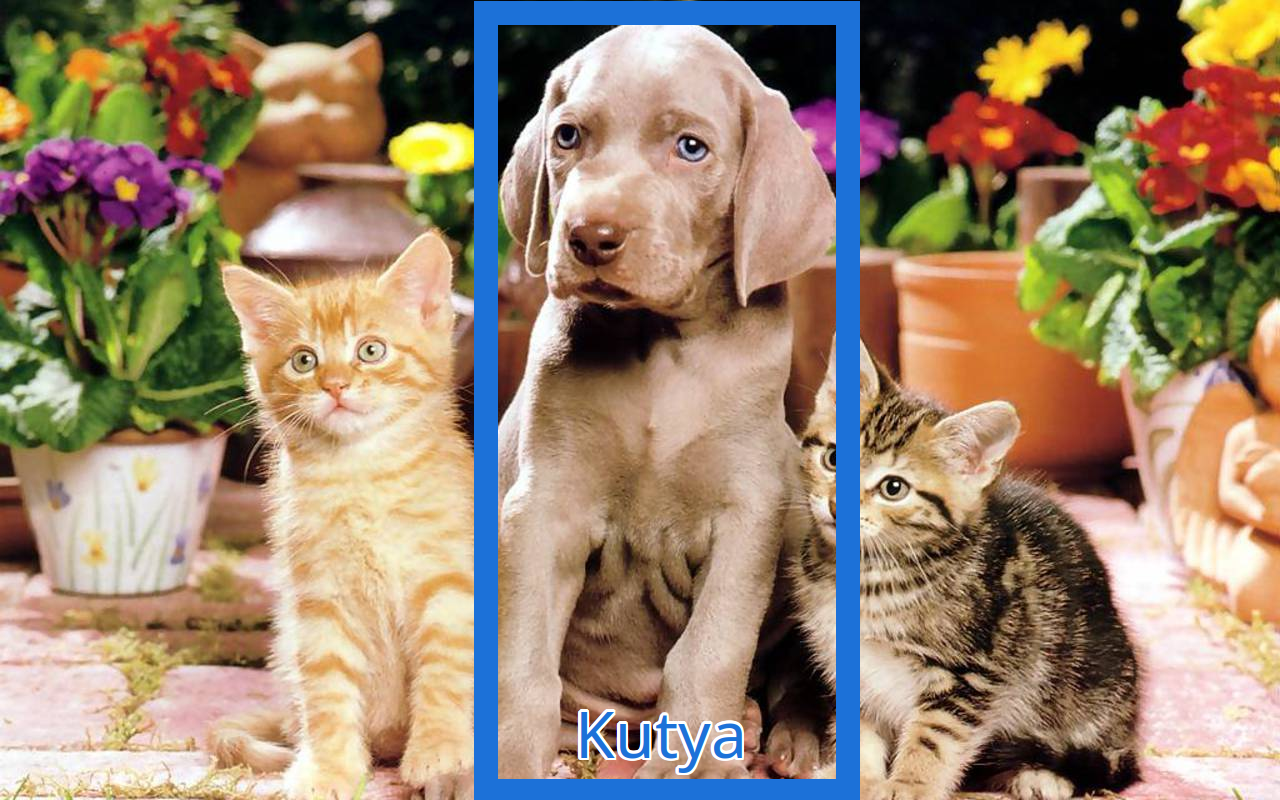
\includegraphics[height=7cm, width=4cm, keepaspectratio]{images/od_7.png}
\end{center}
\end{column}
\end{columns}
\end{frame}

\begin{frame}{Területi javaslatok}
\begin{columns}
\begin{column}{.6\textwidth}
Az eljárás ami meggyorsította a folyamatot a \textbf{területi javaslatok} algoritmusa volt.\par\smallskip
Ahelyett, hogy egy előre meghatározott méretű ablakot csúsztatna végig egy képen, a területi javaslatok algoritmusa megpróbálja a kép \textbf{pixeleit klaszterezni hasonlóság szerint}, ezzel területeket formázva.\par\smallskip
Később ezen \textbf{területeknek a kereteződobozai lesznek átadva egy osztályozó neurális hálózatnak} ami eldönti, hogy a keresett objektumok valamelyike mekkora valószínűséggel található meg a területen.
\end{column}
\begin{column}{.4\textwidth}
\begin{center}
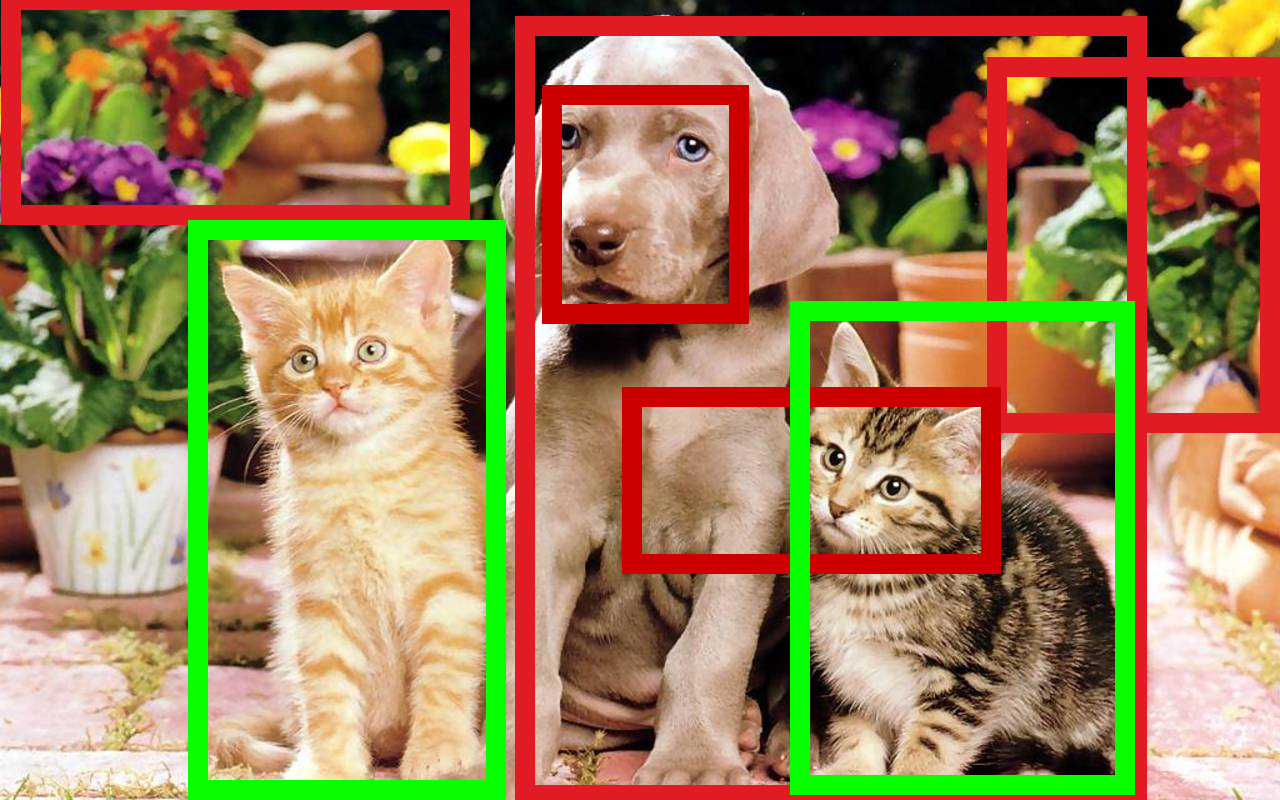
\includegraphics[height=7cm, width=6cm, keepaspectratio]{images/od_8.png}
\end{center}
\end{column}
\end{columns}
\end{frame}

\begin{frame}{Területi javaslatok szelektív kereséssel}
\begin{columns}[T]
\begin{column}{.8\textwidth}
\only<1->{A szelektív keresés egy potenciális objektum területeket javasoló algoritmus, ami jóval hatékonyabban képes működni, mint a csúszóablakos algoritmus:
\begin{enumerate}
	\item \textbf{Kép szegmentálása}: Az input kép pixeleinek csoportosítása szín, textúra és egyéb vizuális tulajdonságok szerint.
	\item \textbf{Régiók hasonlósága}: A különböző régiók összeolvasztása valamilyen hasonlósági mérték szerint.
	\item \textbf{Hierarchikus csoportosítás}: Az összeolvasztott régiók hierarchikus klaszterezése. 
	\item \textbf{Objektum javaslatok}: Objektum javaslatok halmazának elkészítése, amik területi javaslatként szolgálnak.
	\item \textbf{Objektum detekció}: A területi javaslatok átadódnak a neurális hálózatnak osztályozásra.
\end{enumerate}}
\end{column}
\begin{column}{.2\textwidth}
\vspace{-0.5cm}
\begin{center}
\only<1>{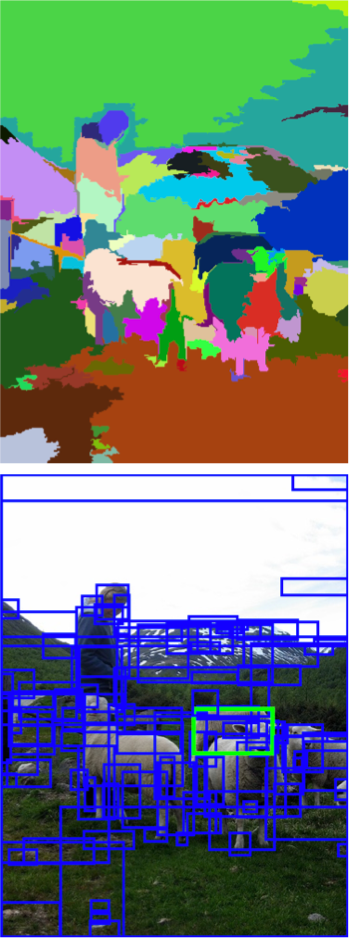
\includegraphics[height=7cm, keepaspectratio]{images/selective_search_1.png}}
\only<2>{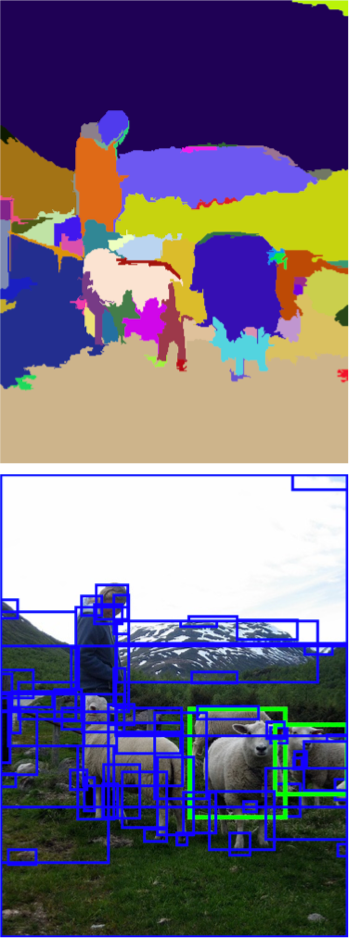
\includegraphics[height=7cm, keepaspectratio]{images/selective_search_2.png}}
\only<3>{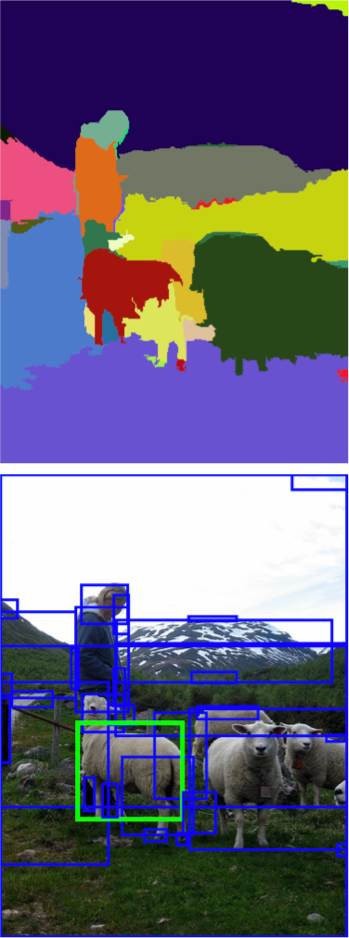
\includegraphics[height=7cm, keepaspectratio]{images/selective_search_3.png}}
\only<4>{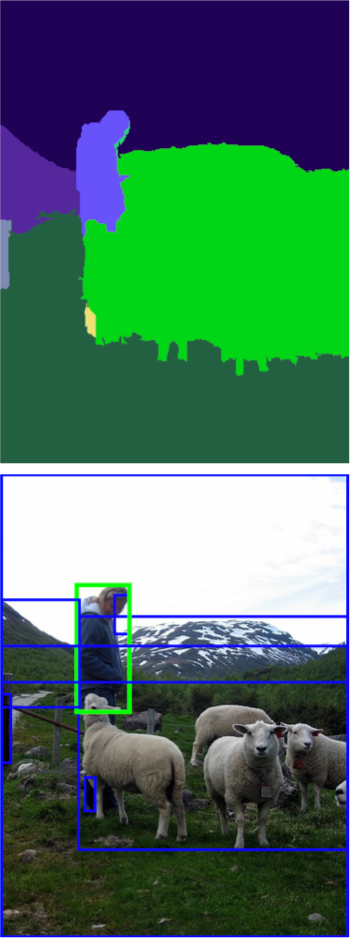
\includegraphics[height=7cm, keepaspectratio]{images/selective_search_4.png}}
\end{center}
\end{column}
\end{columns}
\end{frame}

\begin{frame}{R-CNN architektúra objektum detekcióra}
\begin{columns}
\begin{column}{.4\textwidth}
Az objektum detekció folyamata területjavasolással:
\begin{enumerate}
	\item A területjavasoló \textbf{kiválaszt érdekelt régiókat} a képről. Ezek lehetnek bármekkora méretűek.
	\item A javasolt régiók \textbf{fix méretűre vetítése}. Ez leggyakrabban $224 \cdot 224$ a gyors osztályozás miatt. 
	\item A lokalizációs hálózat \textbf{megbecsüli az osztályokat és a kereteződobozok koordinátáit} a vetített terület alapján.
\end{enumerate}
\end{column}
\begin{column}{.6\textwidth}
\begin{center}
\only<1>{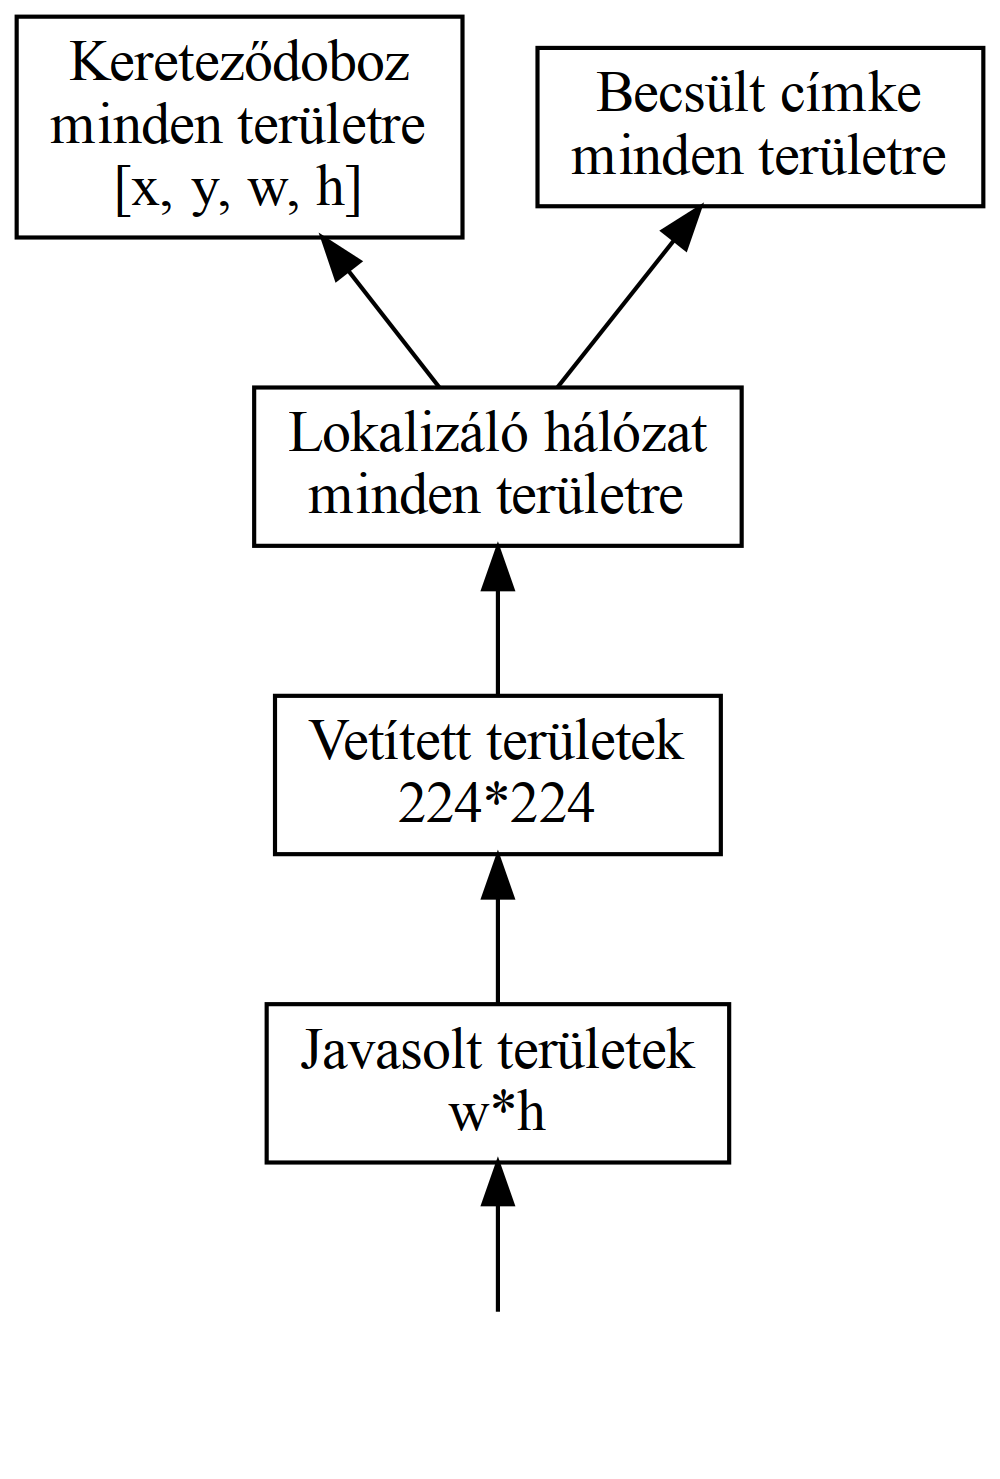
\includegraphics[height=6cm, width=7cm, keepaspectratio]{graphs/od_3.png}\\
\vspace{-0.7cm}
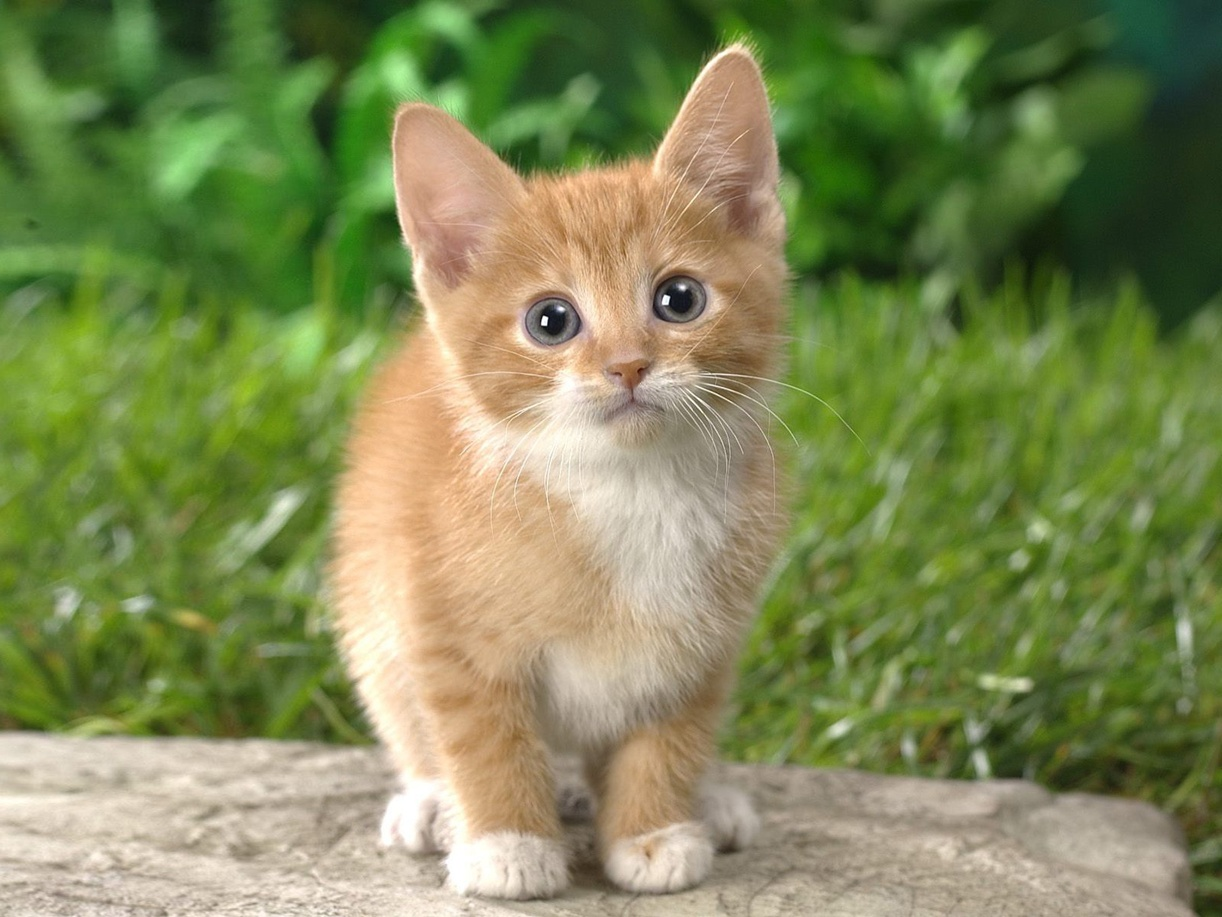
\includegraphics[height=1.5cm, keepaspectratio]{images/od_1.png}}
\only<2>{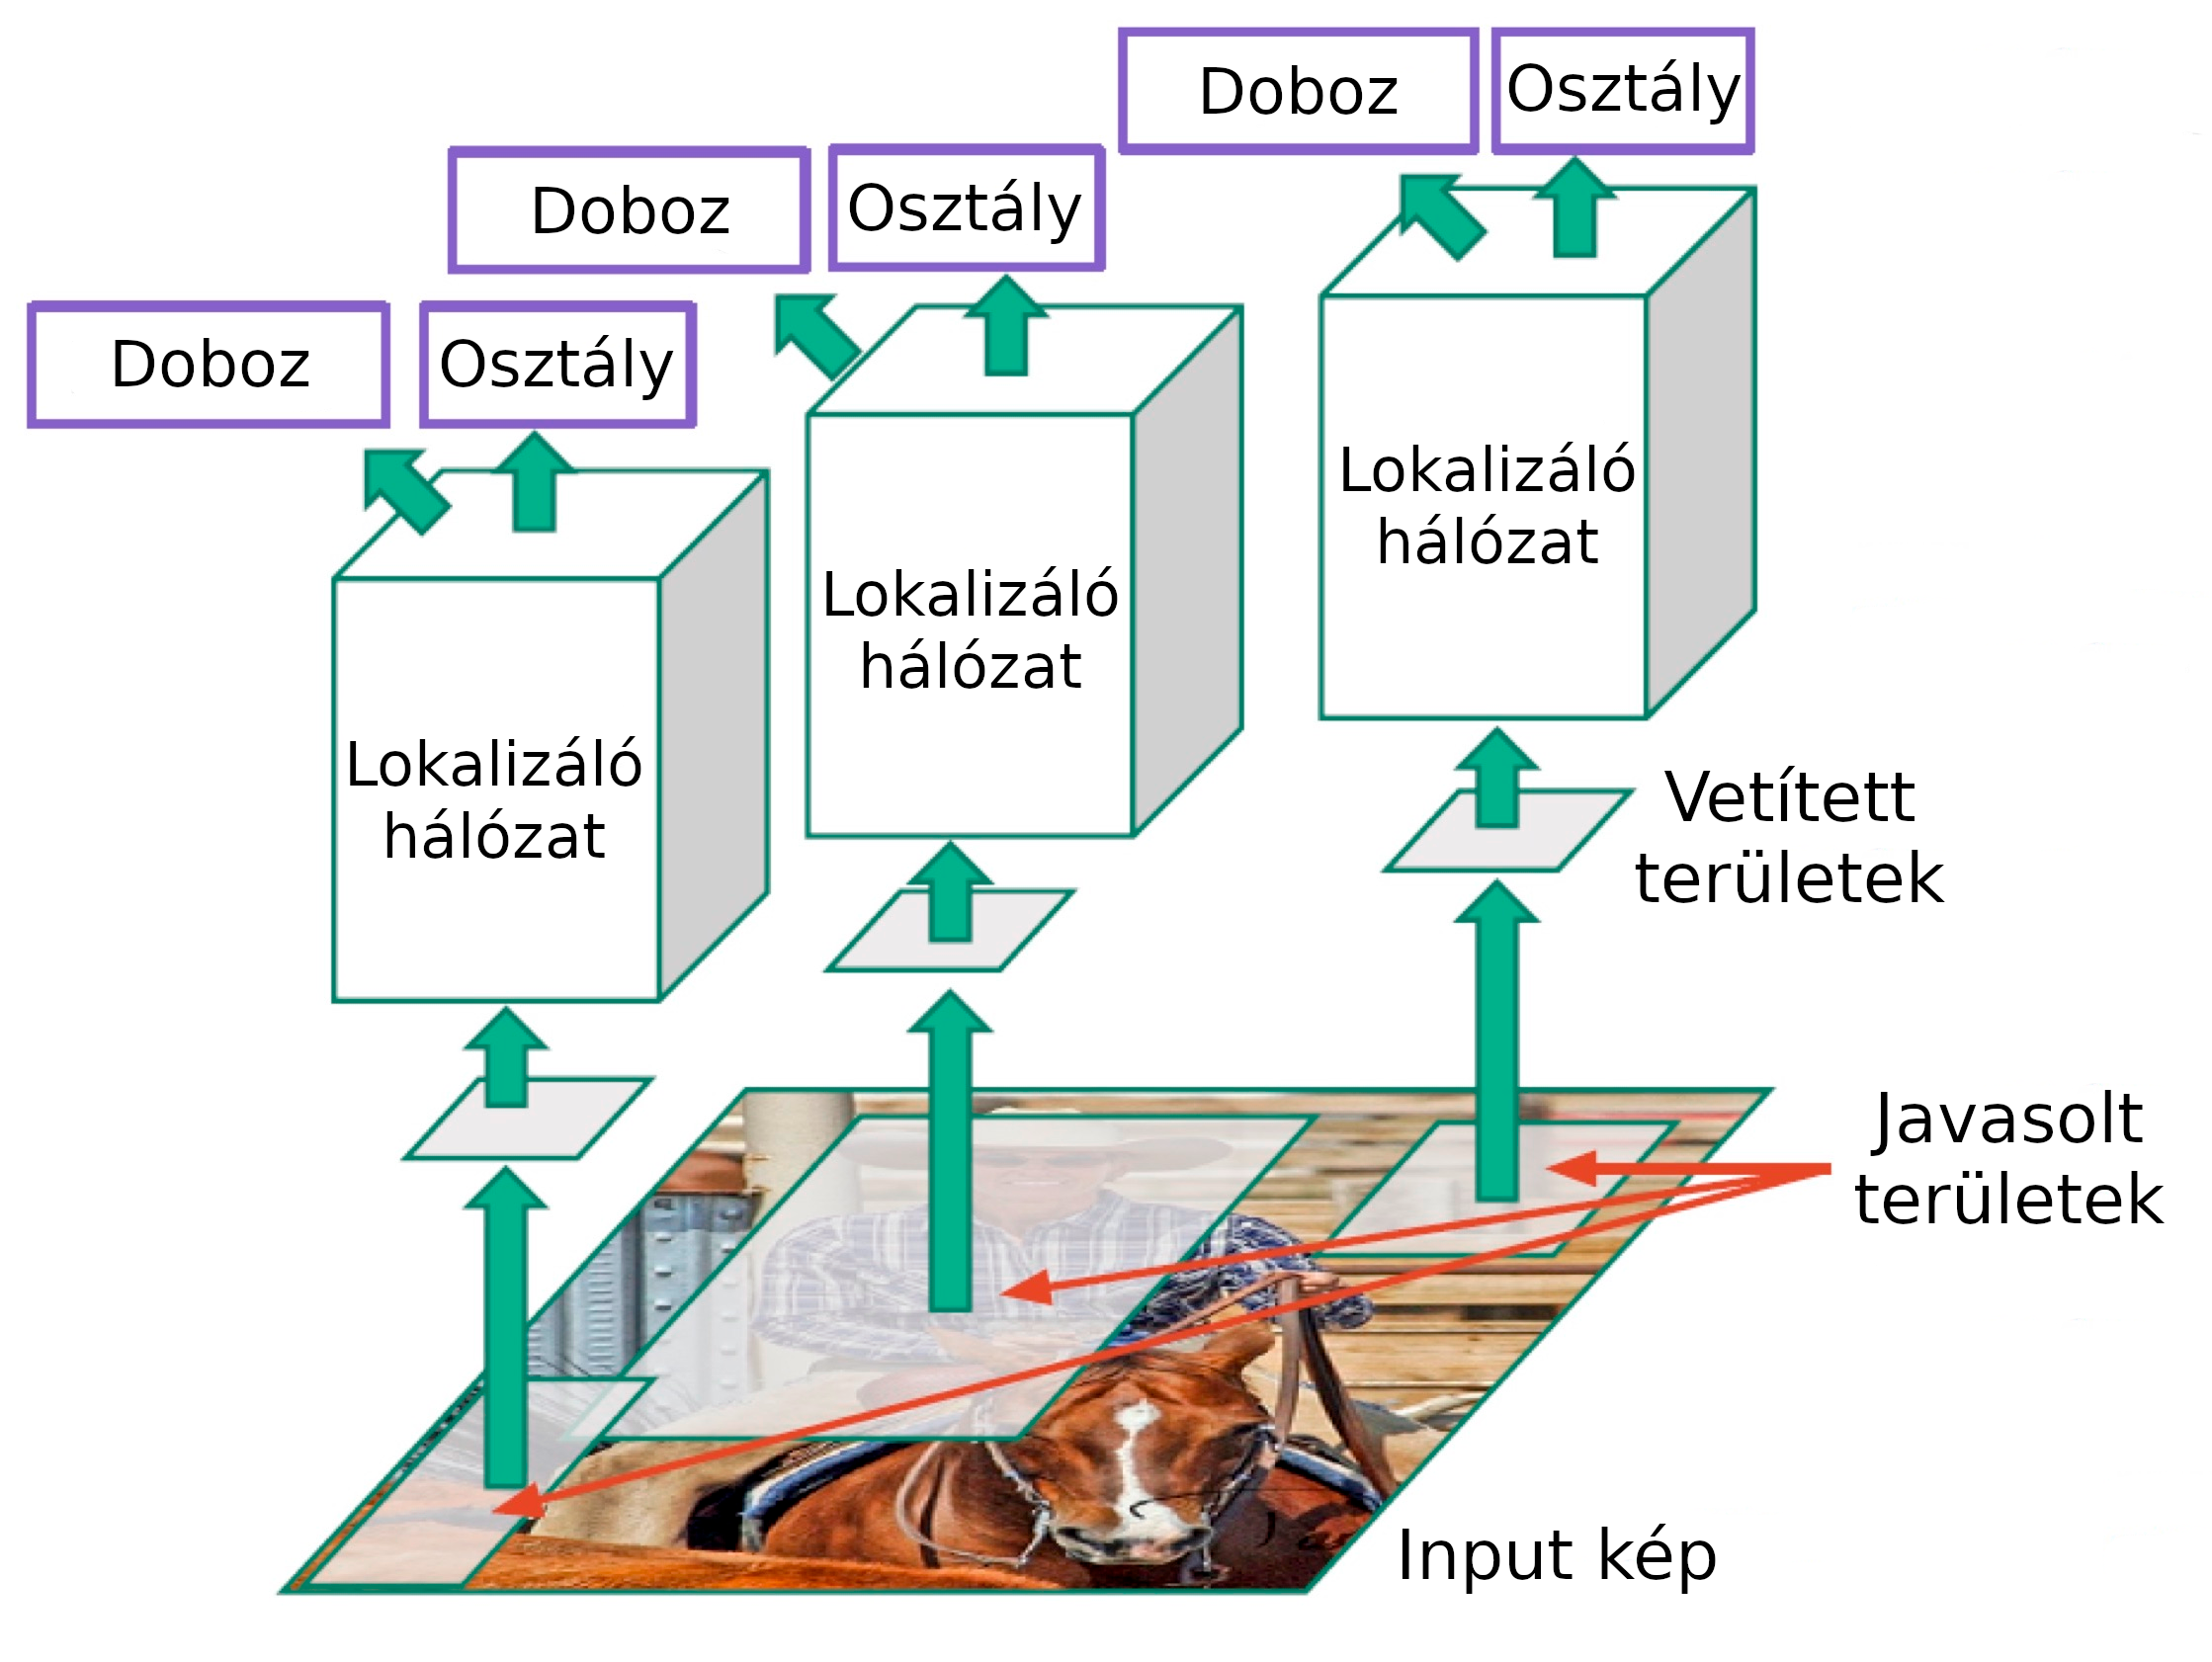
\includegraphics[height=10cm, width=8.5cm, keepaspectratio]{images/od_10.png}}
\end{center}
\end{column}
\end{columns}
\end{frame}

\section{Tanítás}

\begin{frame}
\tableofcontents[currentsection]
\end{frame}

\begin{frame}{Objektum detektció kiértékelése}
\begin{columns}
\begin{column}{.65\textwidth}
A pontosság és visszatérés mérhető objektum detekció esetén is. A \textbf{TP}, \textbf{FP} és \textbf{FN} osztályozás viszont csak specifikusan értelmezhető:
\begin{itemize}
	\item \textbf{TP} (valós pozitív): a becsült osztály megegyezik a valóssal, és $IoU>50\%$.
	\item \textbf{FP} (hamis pozitív): a becsült osztály nem egyezik meg a valóssal \emph{vagy} $IoU<50\%$.
	\item \textbf{FN} (hamis negatív): olyan valós kereteződoboz, amelyikhez nem tartozik predikció.
	\item \textbf{TN} (hamis negatív): nem értelmezett objektum detekció esetén.
\end{itemize}
\end{column}
\begin{column}{.35\textwidth}
\begin{center}
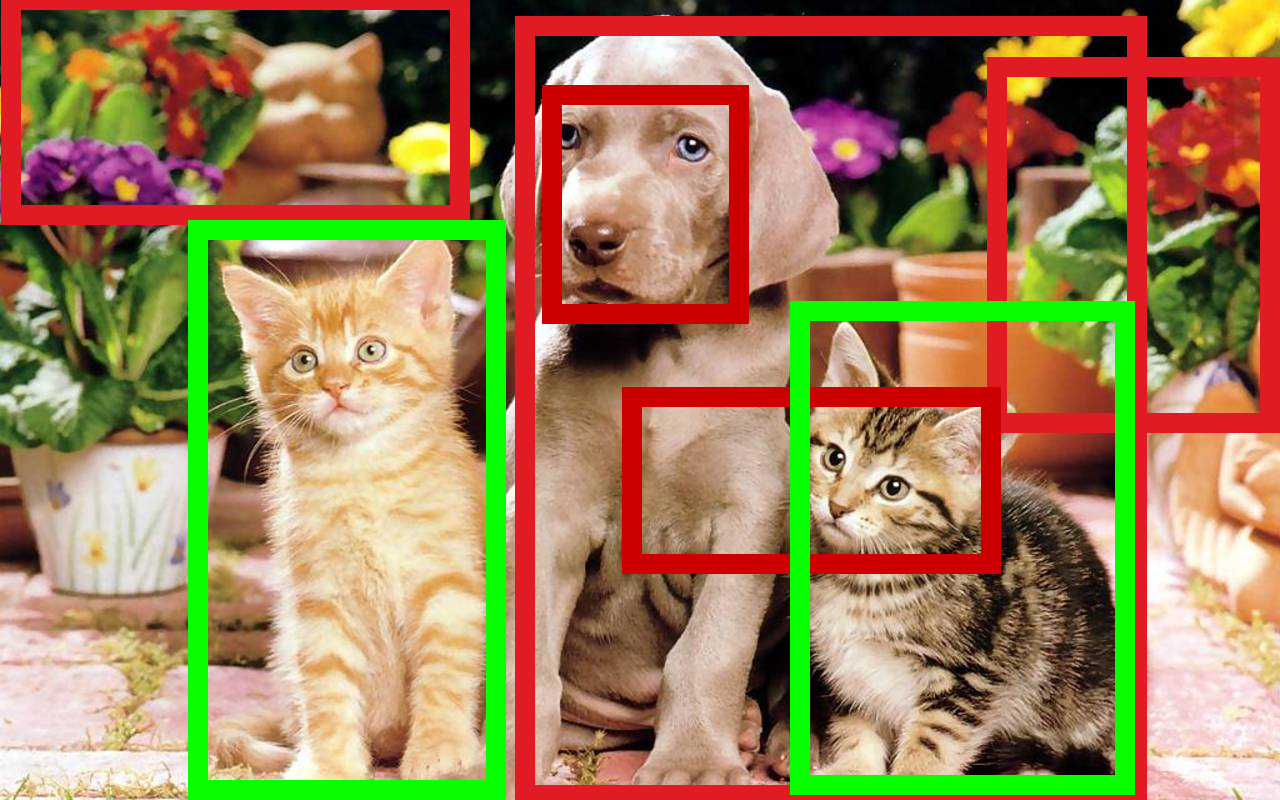
\includegraphics[height=7cm, width=5cm, keepaspectratio]{images/od_8.png}
\end{center}
\end{column}
\end{columns}
\end{frame}

\begin{frame}{Az objektum detekció mérőszámai}
\begin{columns}
\begin{column}{.5\textwidth}
A detekció pontosságának két fontos mutatója:
\begin{itemize}
	\item \textbf{Pontosság}: A megbecsült elemek közül hány volt valós pozitív? 
	\[
	P=\frac{TP}{TP+FP}
	\]
	\item \textbf{Visszahívás}: A valós pozitívak közül hány elem lett megbecsülve? 
	\[
	R=\frac{TP}{TP+FN}
	\]
\end{itemize}
\end{column}
\begin{column}{.5\textwidth}
\begin{center}
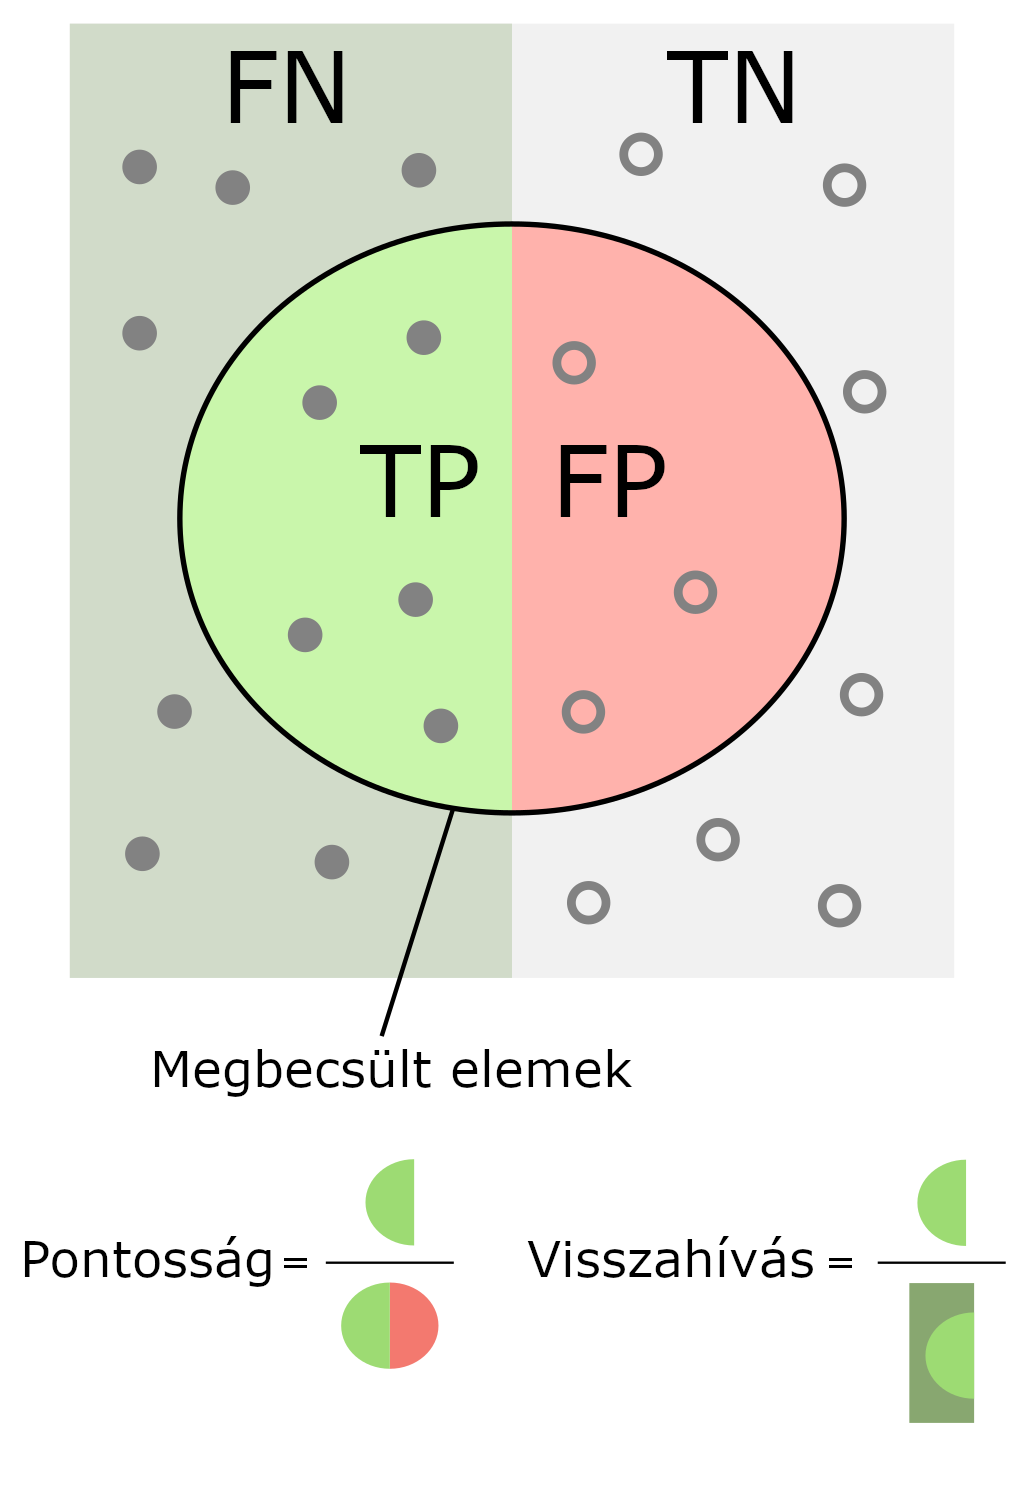
\includegraphics[width=7cm, height=7cm, keepaspectratio]{images/od_11.png}
\end{center}
\end{column}
\end{columns}
\end{frame}

\begin{frame}{Átlagos pontosság}
\begin{columns}
\begin{column}{.5\textwidth}
Az átlagos pontosság a pontosság-visszahívás görbe alatti terület. 
\begin{block}{Átlagos pontosság (AP)}
Az átlagos pontosság a pontossági értékek súlyozott átlaga minden pontossági küszöbértéken kiértékelve:
\[
AP = \frac{1}{n} \sum_{R=0}^1 P(R)
\]
Ahol $n$ a mintavételi gyakoriság, $P(\cdot)$ a pontosság és $R$ a visszahívás értéke. Az $R$ küszöbérték $n$ db értéket vesz fel $0$ és $1$ között. 
\end{block}
\end{column}
\begin{column}{.5\textwidth}
\begin{center}
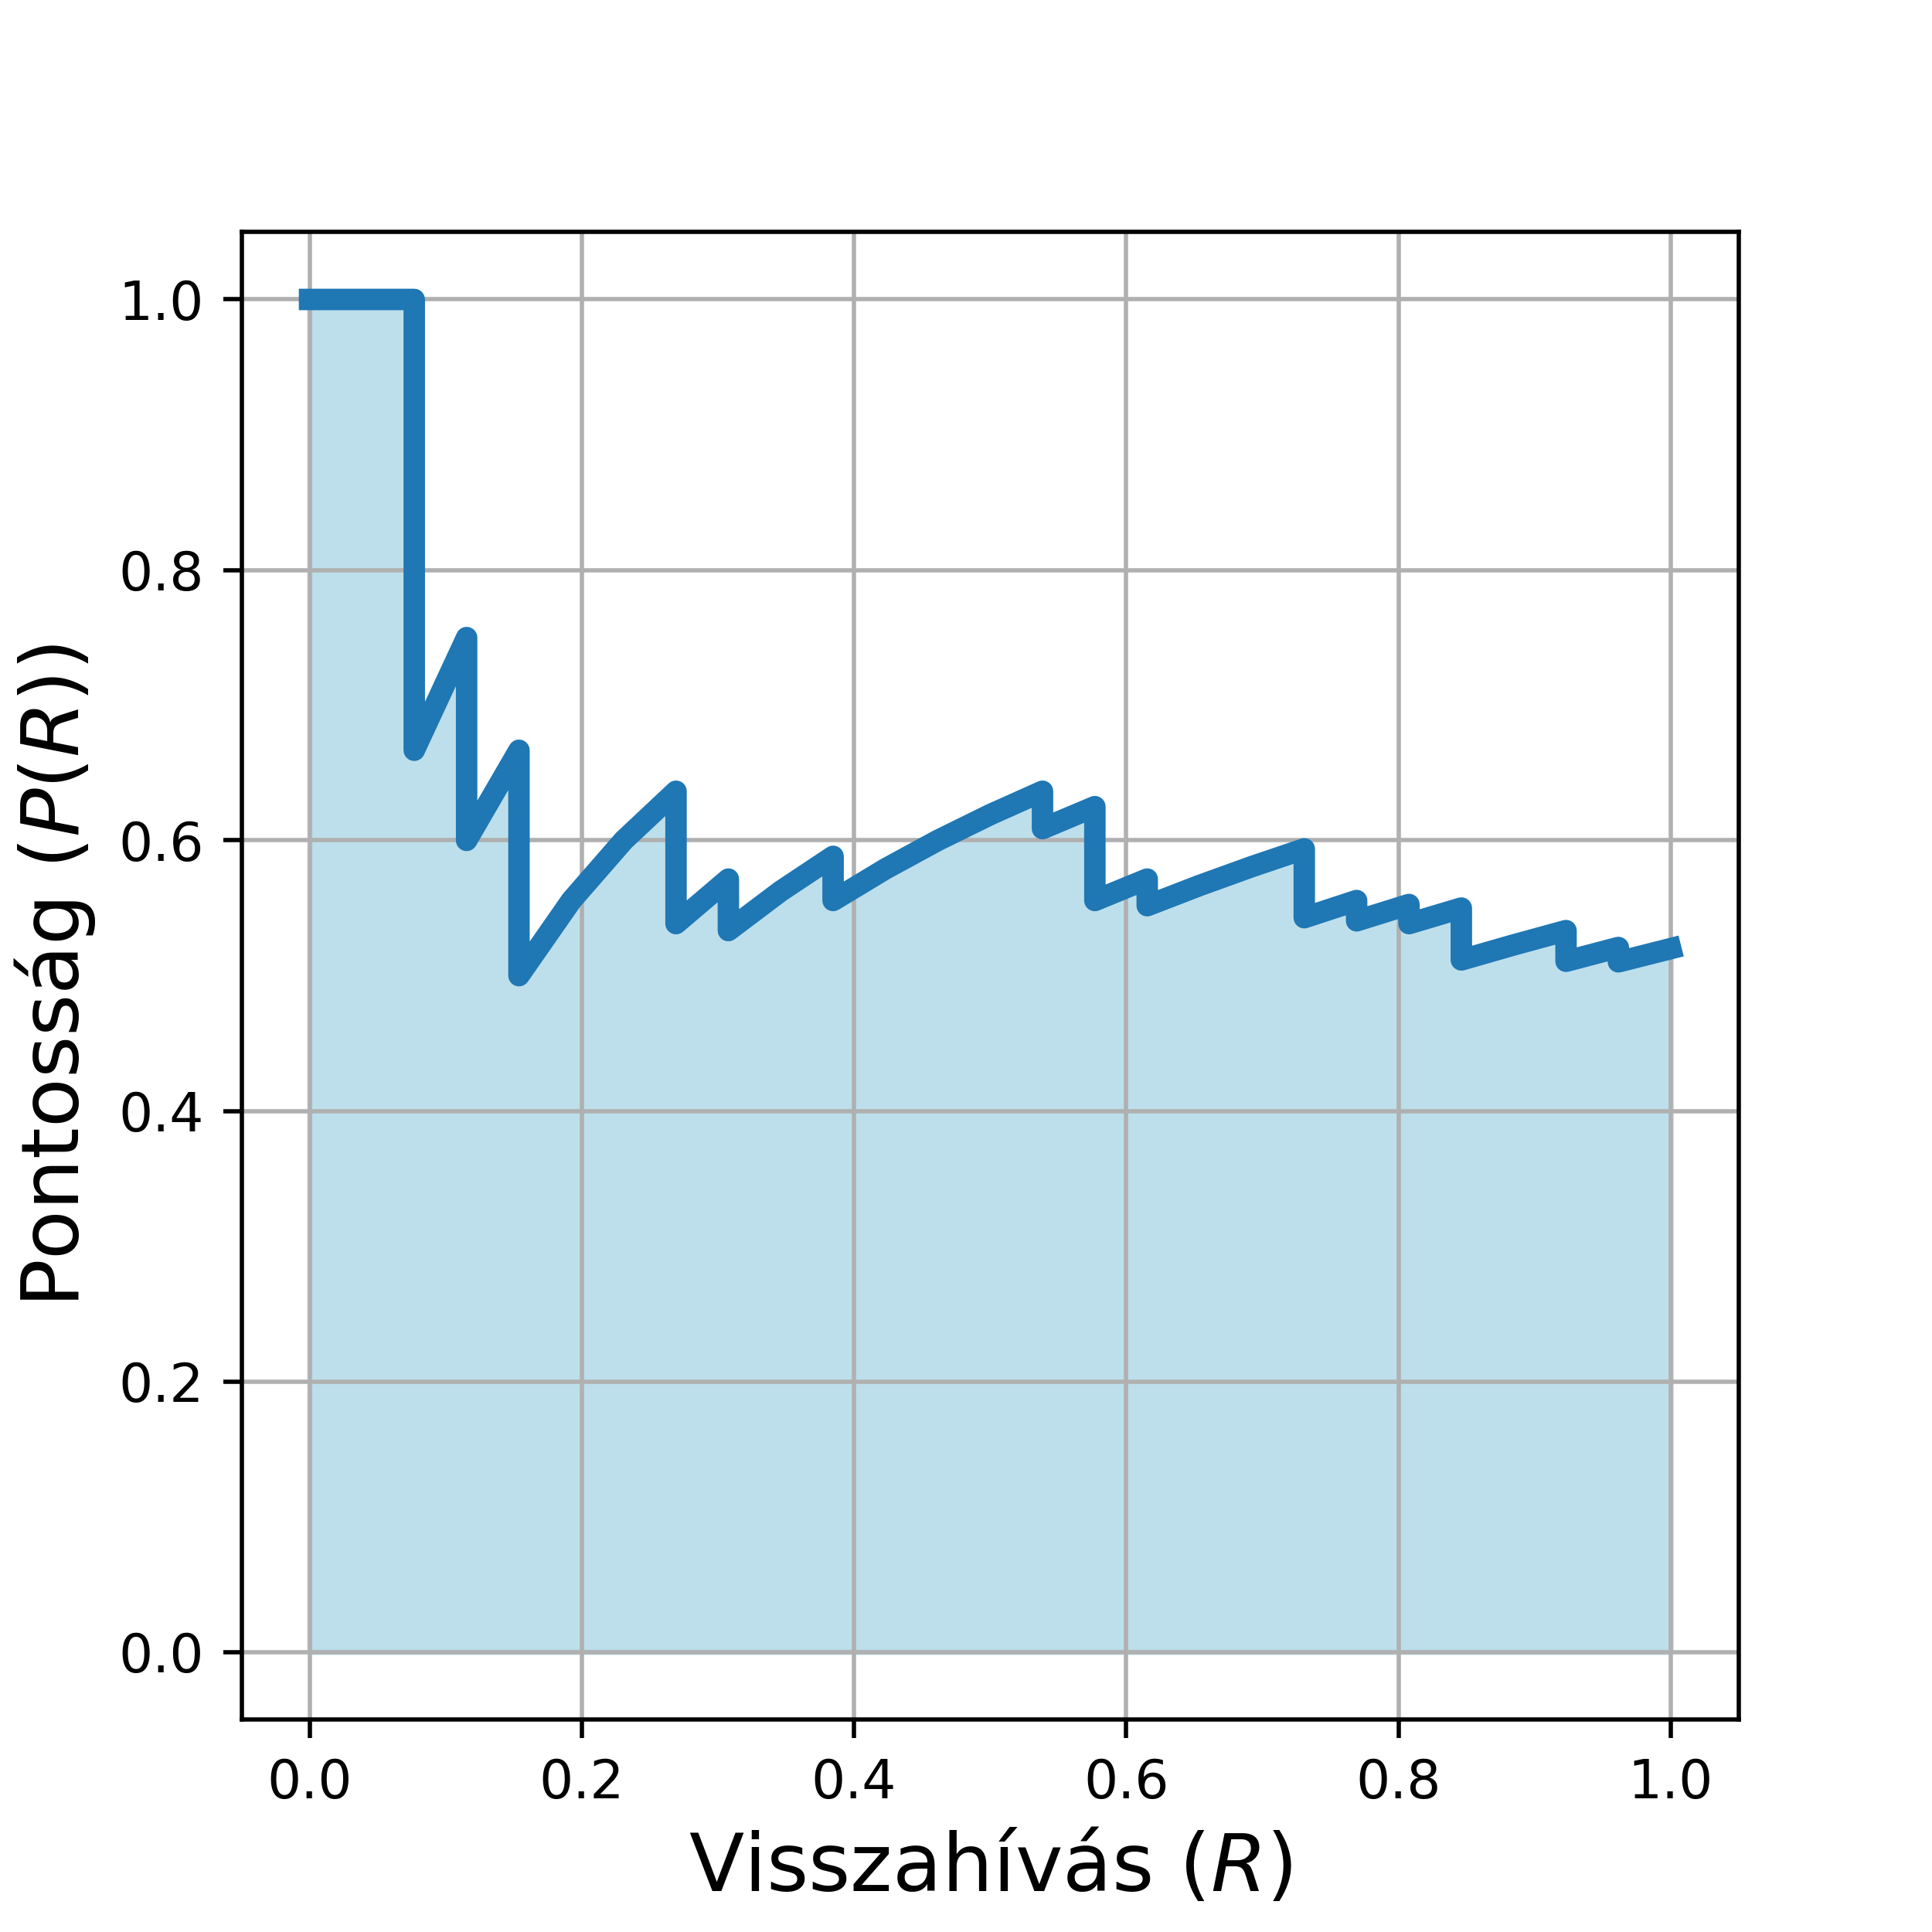
\includegraphics[width=7cm, keepaspectratio]{images/od_12.png}
\end{center}
\end{column}
\end{columns}
\end{frame}

\begin{frame}{Közepes átlagos pontosság}
\begin{columns}
\begin{column}{.5\textwidth}
\begin{block}{Közepes átlagos pontosság (mAP)}
A közepes átlagos pontosság az összes osztályra kiszámított átlagos pontosságok átlaga:
\[
mAp = \frac{1}{N} \sum_{i=0}^{N-1} AP_i = \frac{1}{N} \sum_{i=0}^{N-1} \frac{1}{n} \sum_{R=0}^1 P_i(R)
\]
Ahol $N$ az oszályok számossága, $n$ a küszöbértékeni mintavételek száma, $AP_i$ az átlagos pontosság  az $i$. osztályra.
\end{block}
\end{column}
\begin{column}{.5\textwidth}
\begin{center}
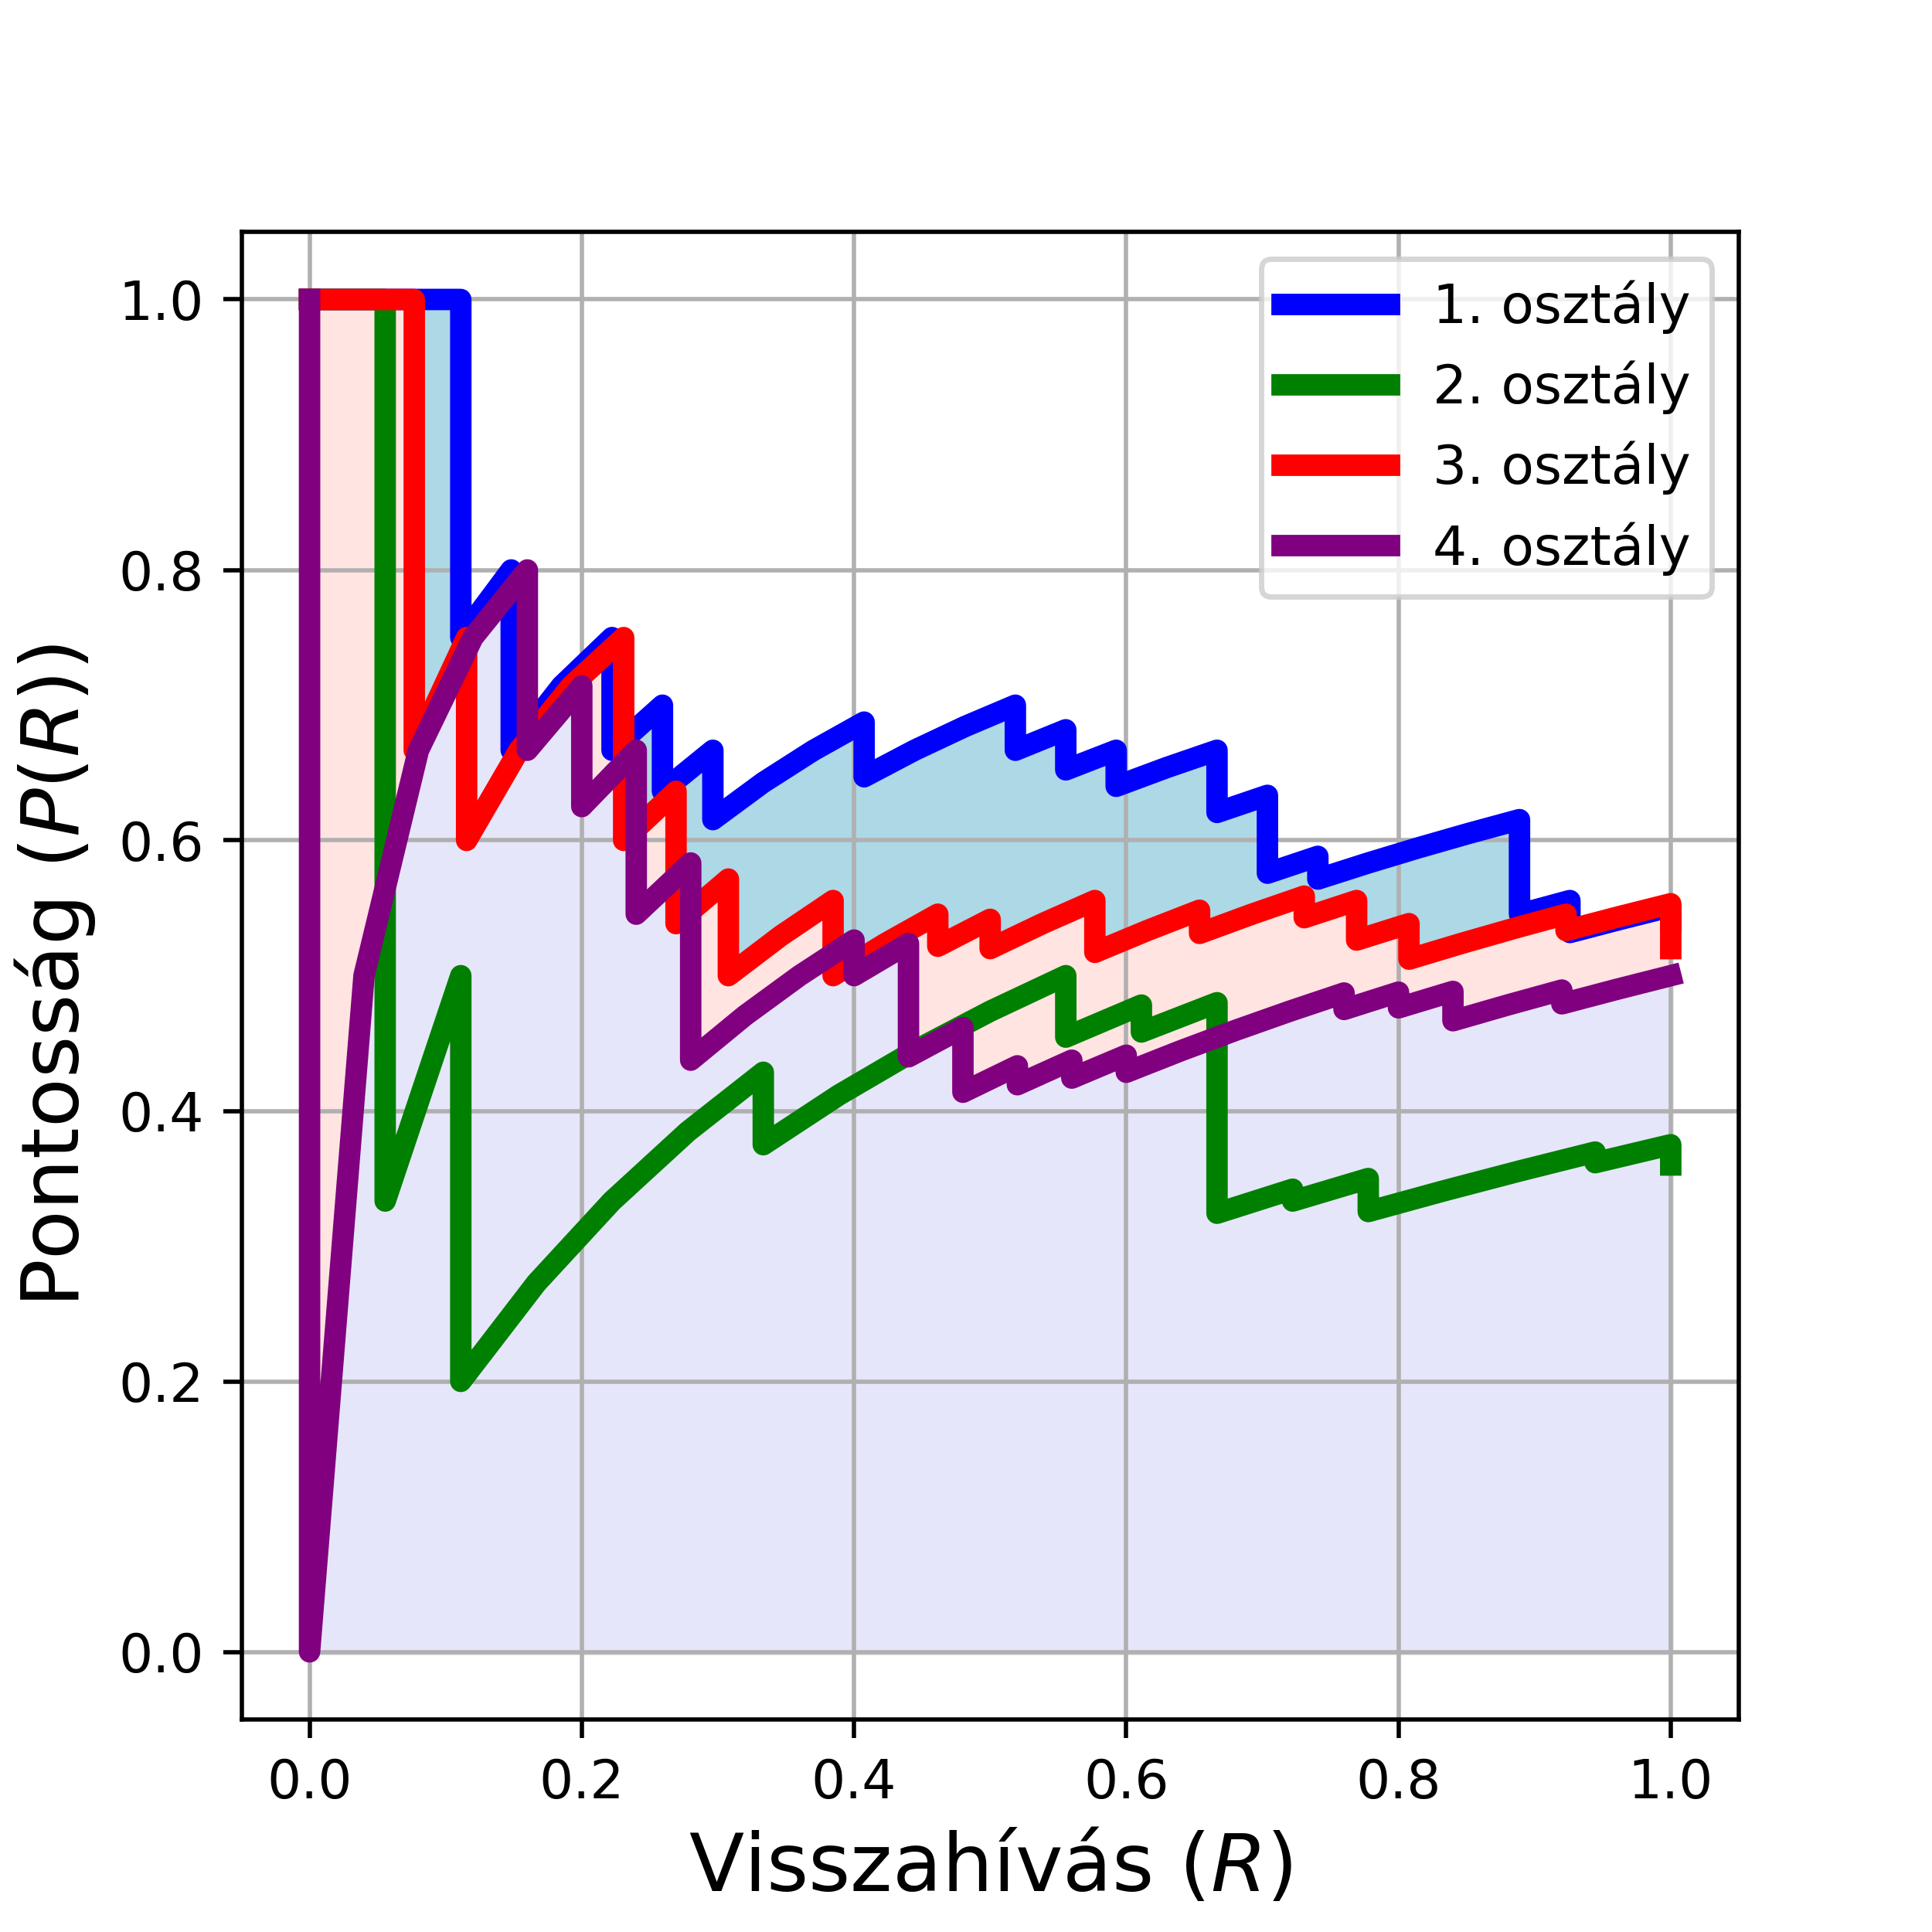
\includegraphics[width=7cm, keepaspectratio]{images/od_13.png}
\end{center}
\end{column}
\end{columns}
\end{frame}

\begin{frame}{Térbeli piramis lazítás}
\begin{columns}
\begin{column}{.5\textwidth}
Térbeli piramis pooling (SPP) réteg az inputot \textbf{több, különböző méretű max pooling réteggel dolgozza fel}. Például ha érkezik egy konvolúciós rétegból valamilyen aktiváció feldolgozza egy $1 \cdot 1$, $2 \cdot 2$ és $4 \cdot 4$ max pooling szűrővel is.\par\smallskip
Ha a piramis pooling réteg után egy teljesen becsatolt réteg következik, a különböző pooling rétegek által adott \textbf{outputot kilapítja, konkatenálja majd úgy adja tovább} a következő rétegnek.\par\smallskip
Lapítás során az input mátrixból 1 dimenziós vektor lesz. Pl. $4 \cdot 4 \rightarrow 16 \cdot 1$.
\end{column}
\begin{column}{.5\textwidth}
\begin{center}
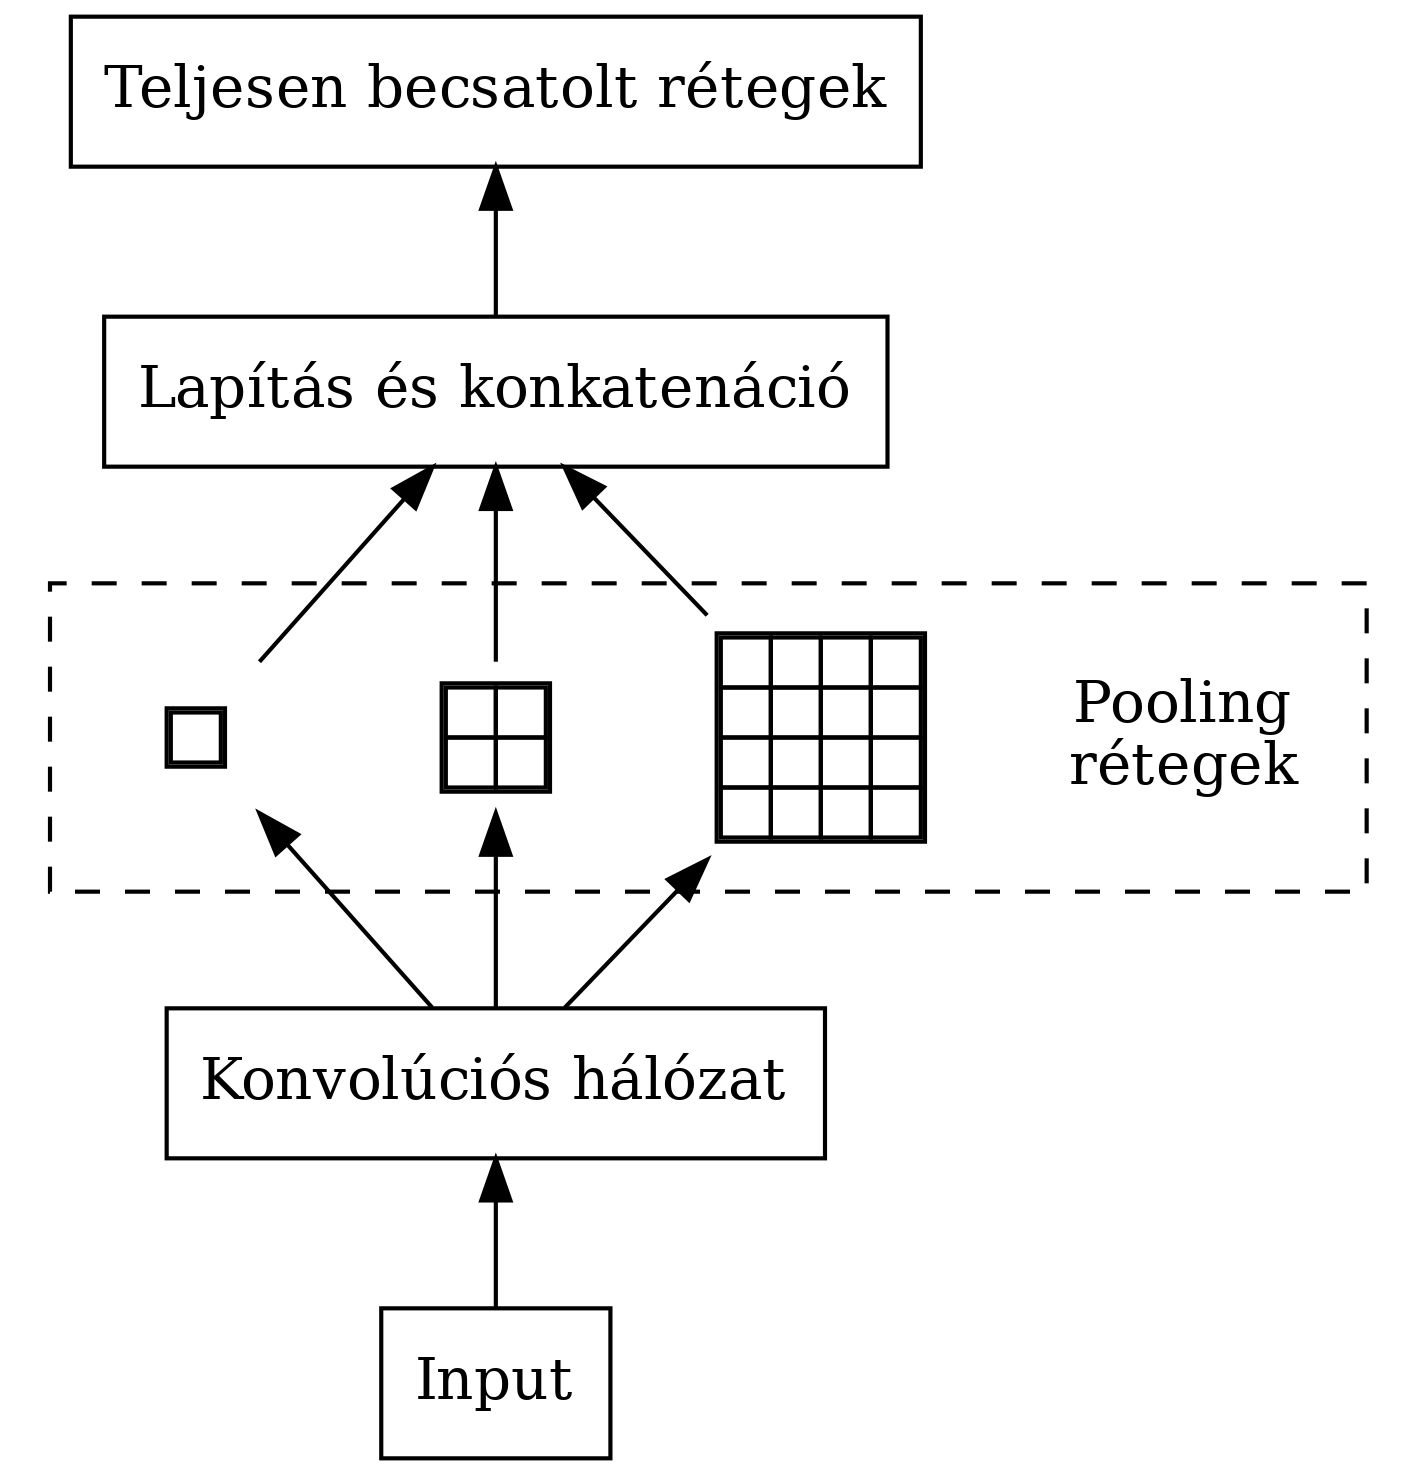
\includegraphics[height=7cm, keepaspectratio]{graphs/od_4.png}
\end{center}
\end{column}
\end{columns}
\end{frame}

\section{További architektúrák}

\begin{frame}
\tableofcontents[currentsection]
\end{frame}

\begin{frame}{Fast R-CNN}
\begin{columns}
\begin{column}{.4\textwidth}
Az eredeti R-CNN architektúra nagyon lassan futott, hiszen a sok műveletet igénylő konvolúciós szűrés \textbf{minden javasolt érdekelt területre lefutott}.\par\smallskip
A Fast-RCNN az eredeti architektúrát úgy módosítja, hogy \textbf{először a konvolúciós rétegeken áramoltatja át az input adatot}, majd a konvolúciós rétegek outputján keresi meg az érdekelt területeket, amiket vetít és beosztályoz a régióalapú hálózattal.
\end{column}
\begin{column}{.6\textwidth}
\only<1>{
\begin{center}
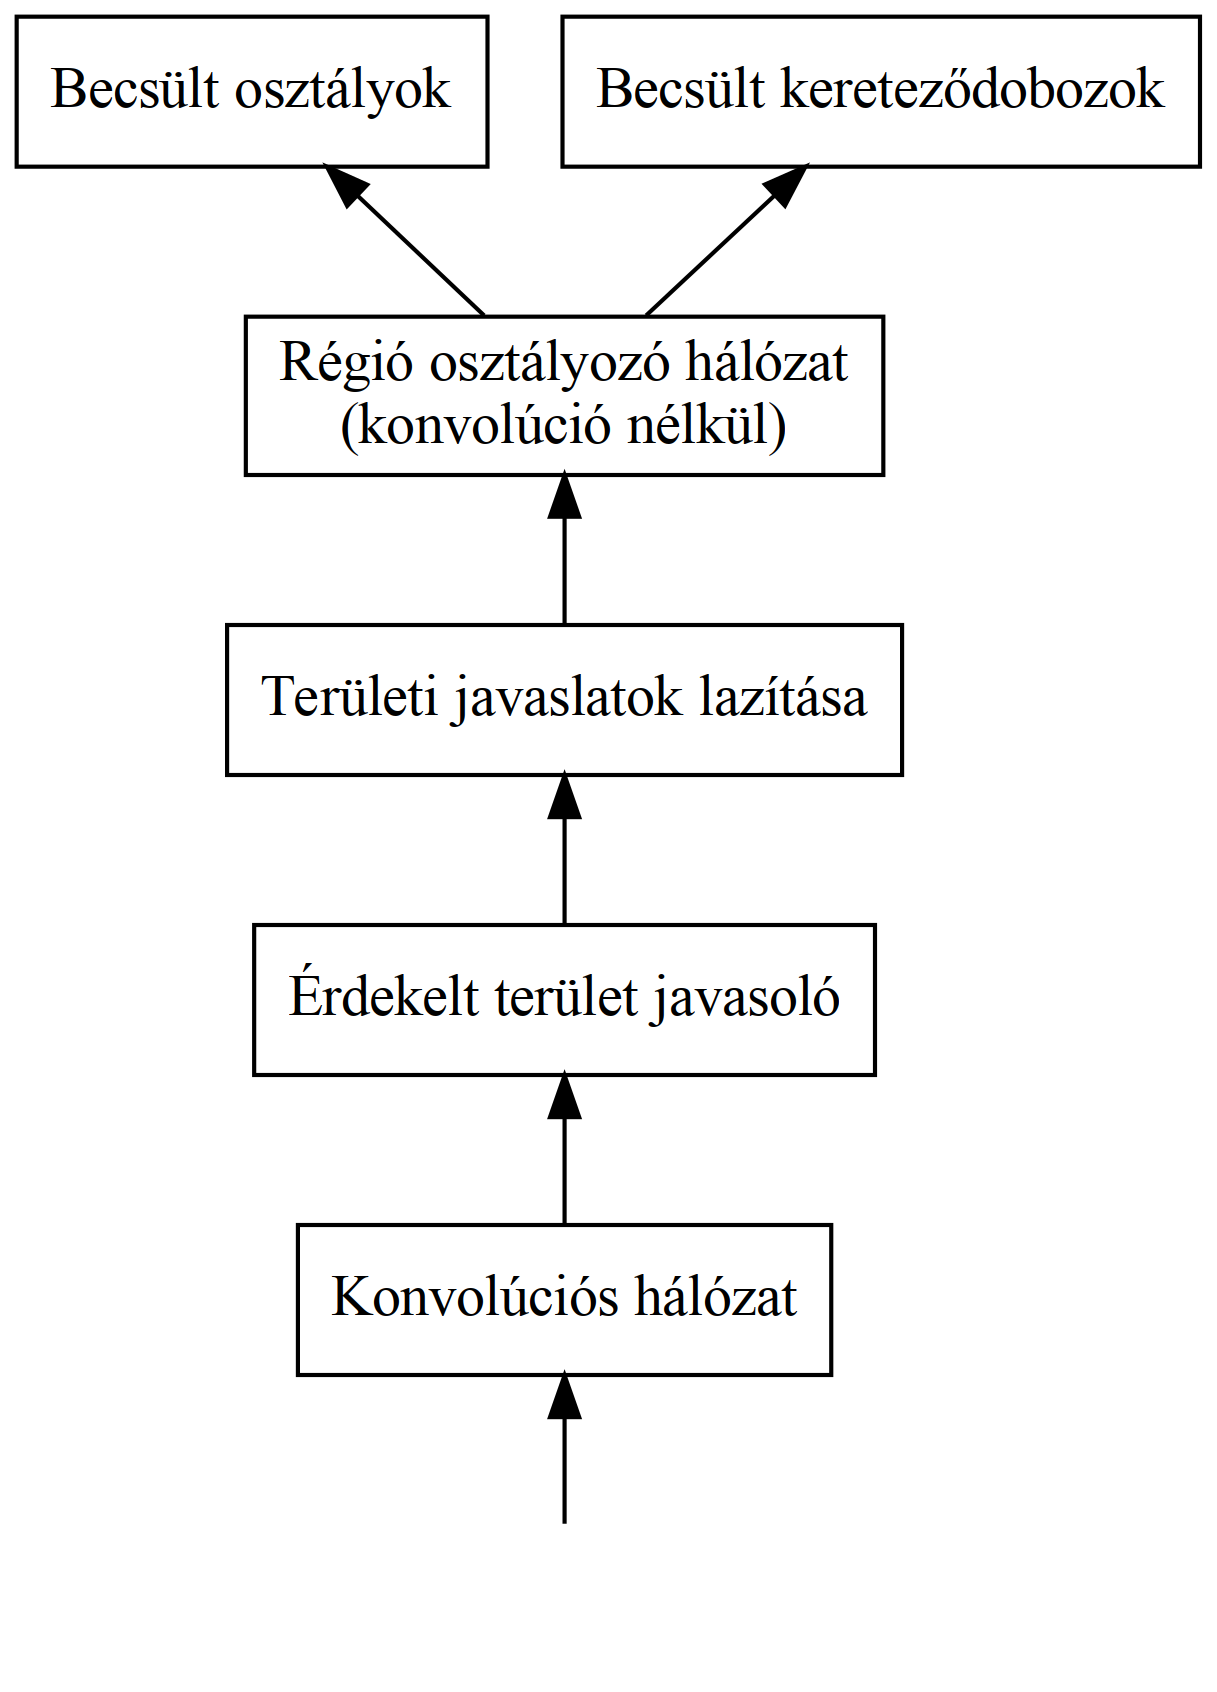
\includegraphics[height=6cm, keepaspectratio]{graphs/od_5.png}\\
\vspace{-0.7cm}
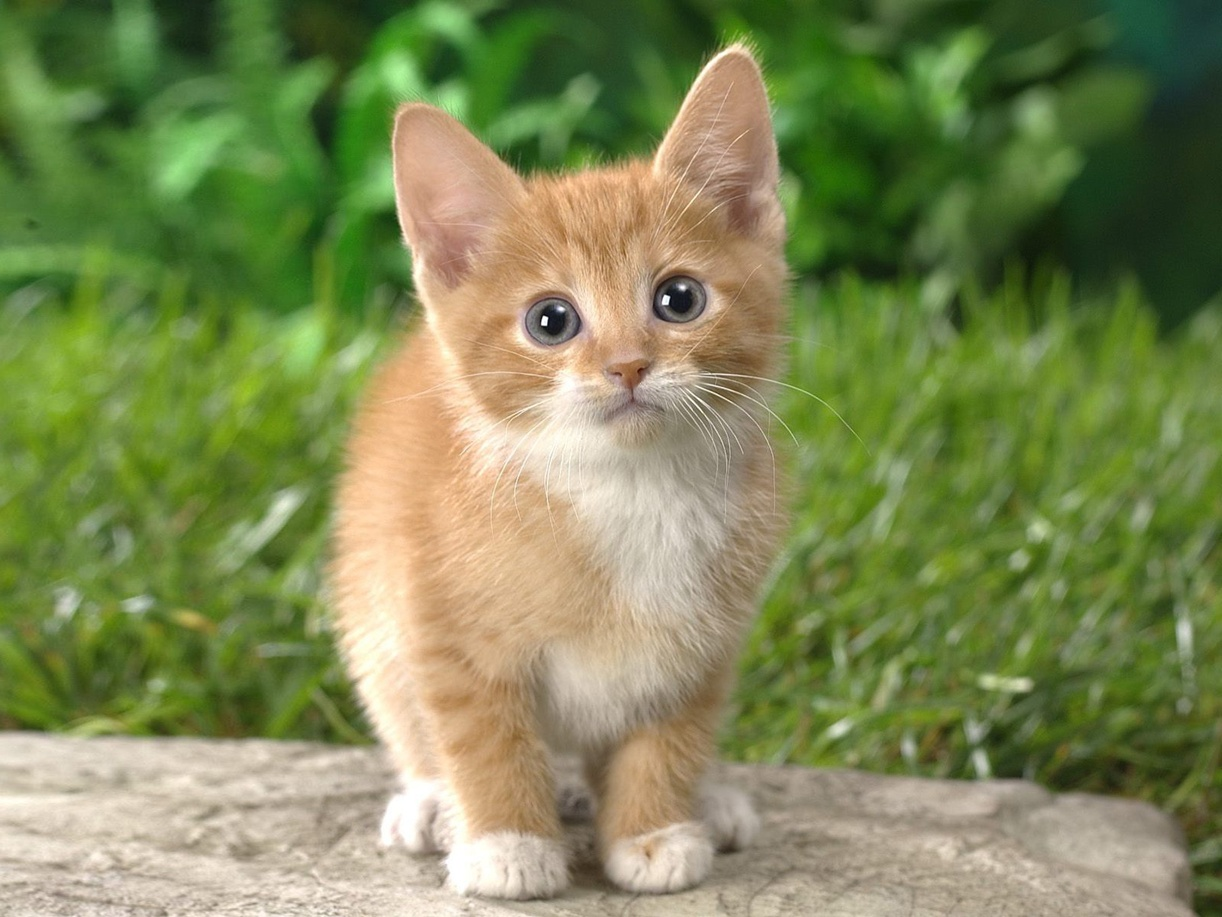
\includegraphics[height=1.5cm, width=2.5cm, keepaspectratio]{images/od_1.png}
\end{center}}
\only<2>{
\begin{center}
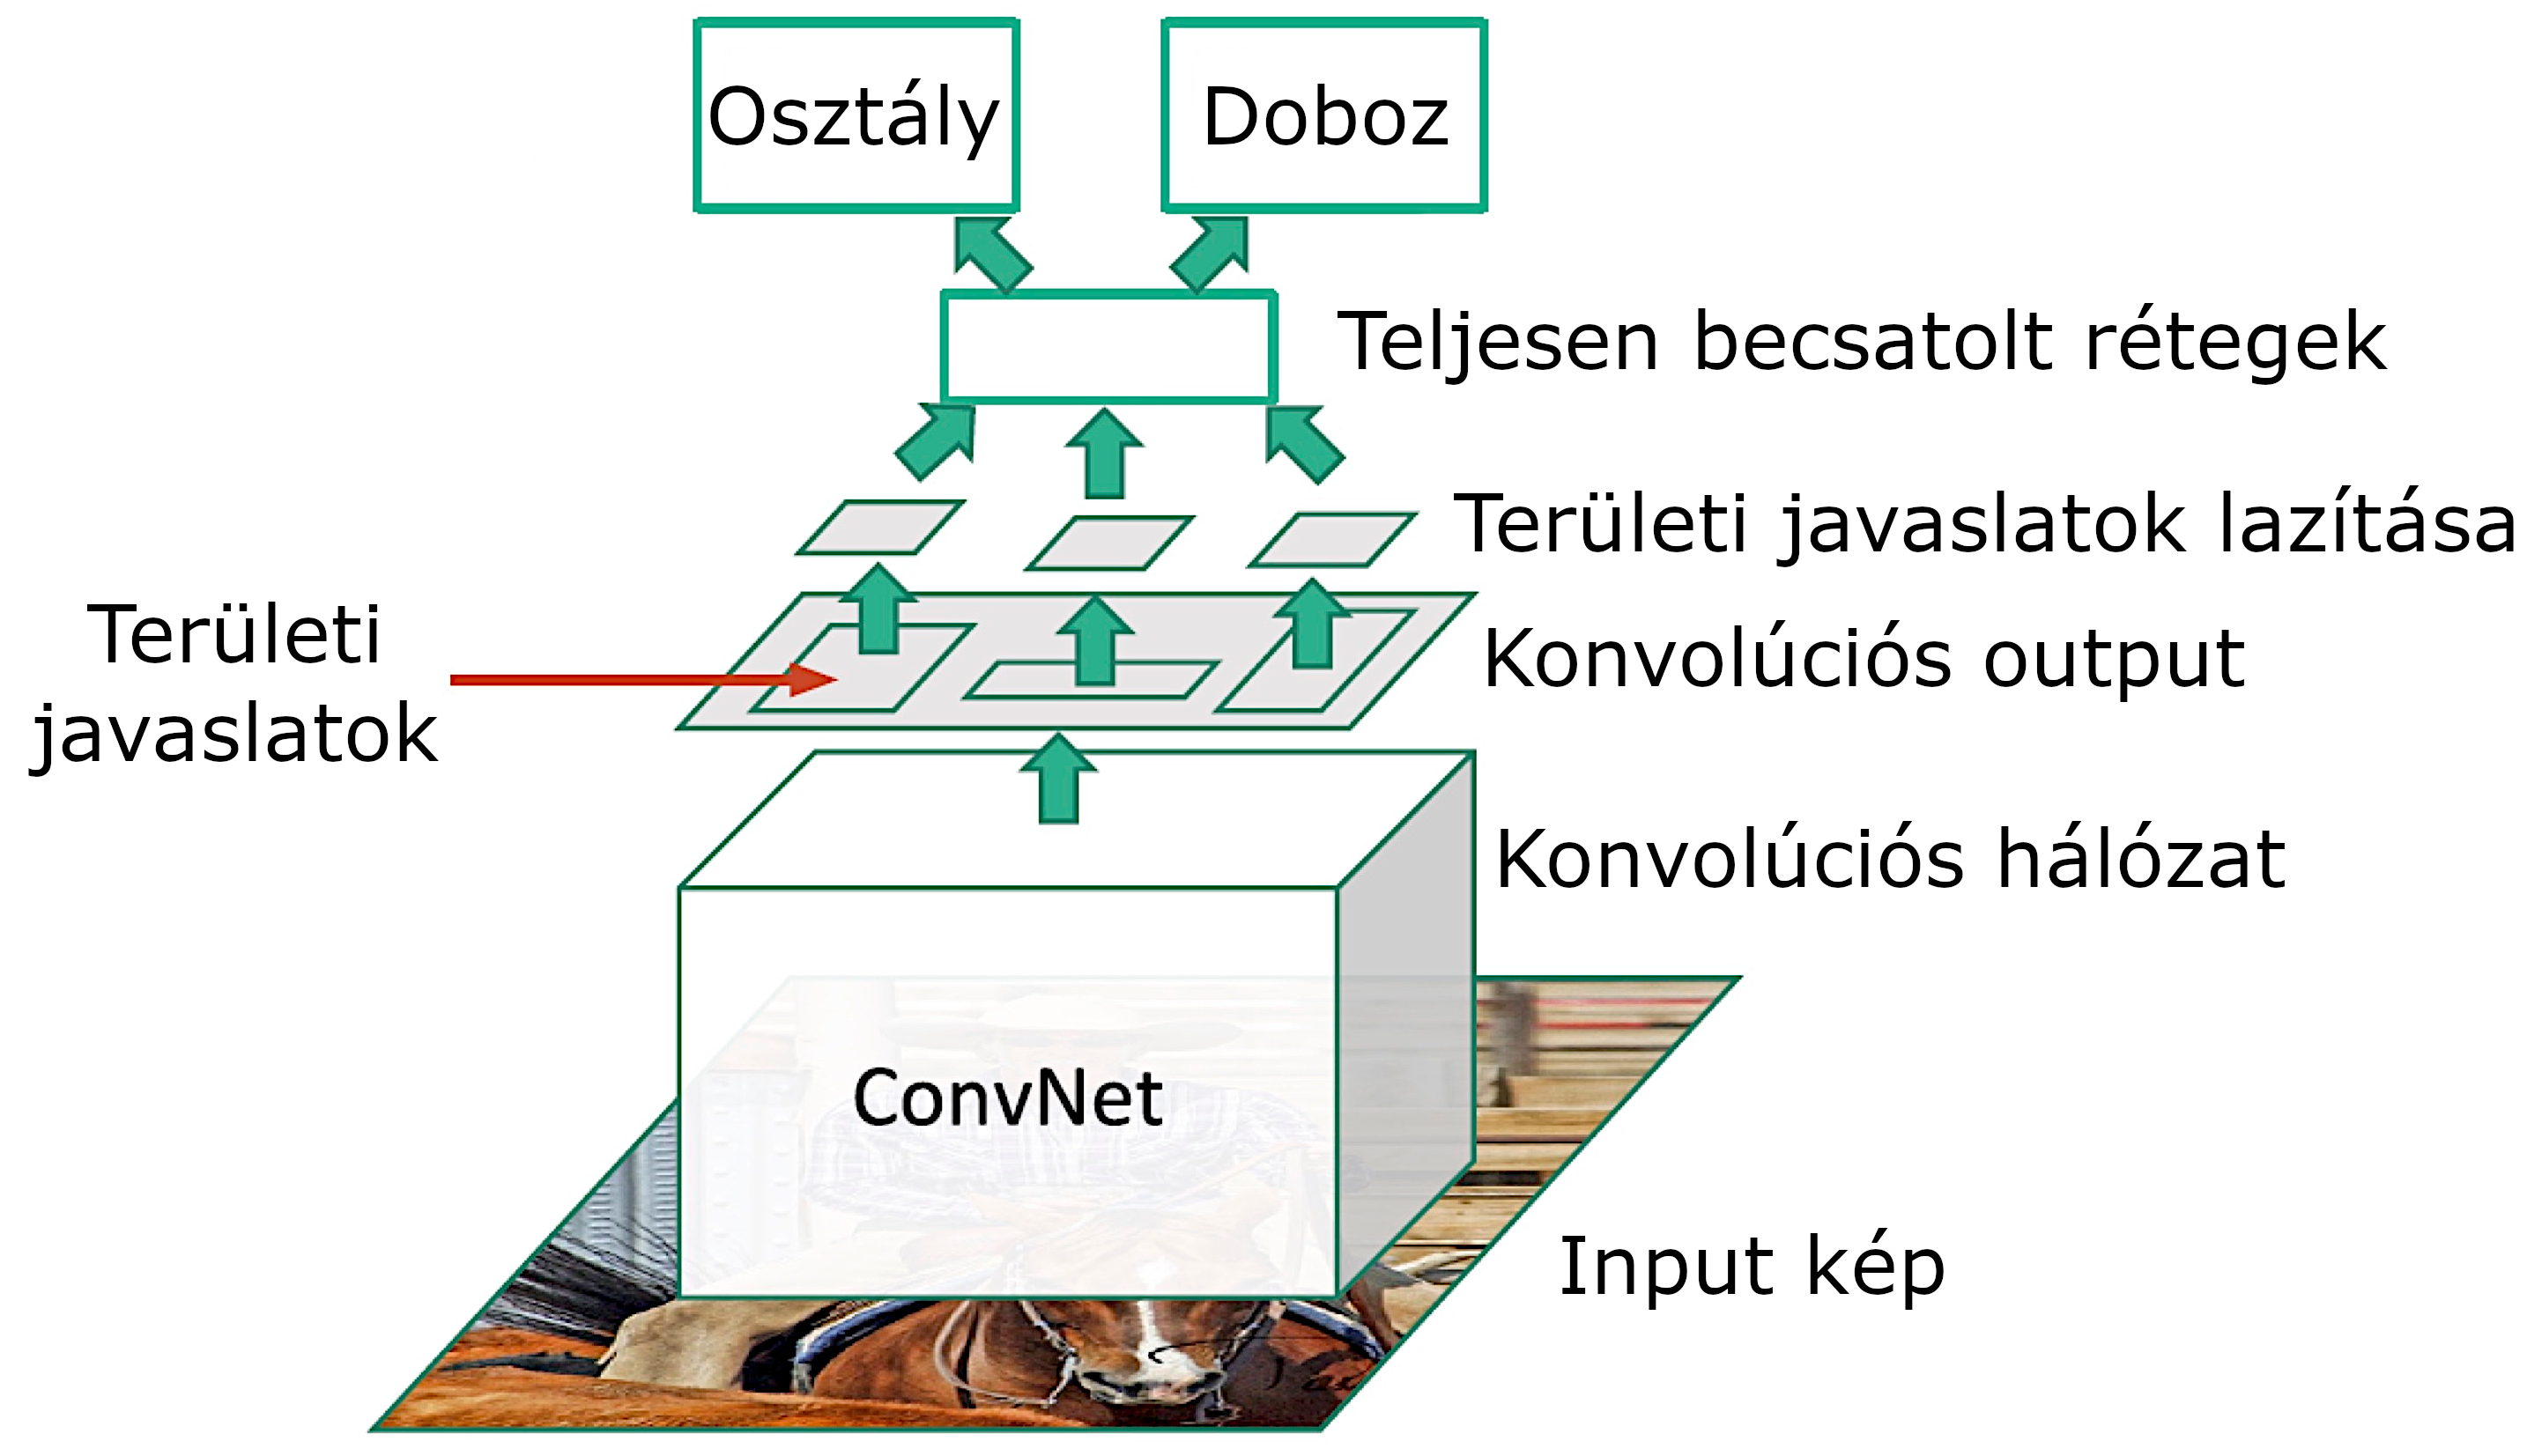
\includegraphics[width=9cm, height=7cm, keepaspectratio]{images/od_14.png}
\end{center}}
\end{column}
\end{columns}
\end{frame}

\begin{frame}{Területi javaslatok lazítása (RoI pooling)}
\begin{columns}
\begin{column}{.5\textwidth}
A területenkénti konvolúciós hálózatk \textbf{fix méretű inputot} várnak a korábbi rétegektől, viszont a területi javaslatok eltérő méretűek.\par\smallskip
Ebből adódóan szükség van a területi javaslatok átméretezésére. A RoI pooling réteg feladata \textbf{fix méretű mátrixokká transzformálni} a bemeneti mátrixokat.\par\smallskip
Például egy RoI pooling réteg kimenete bármilyen méretű mátrixra lehet $224 \cdot 224$.
\end{column}
\begin{column}{.5\textwidth}
\begin{center}
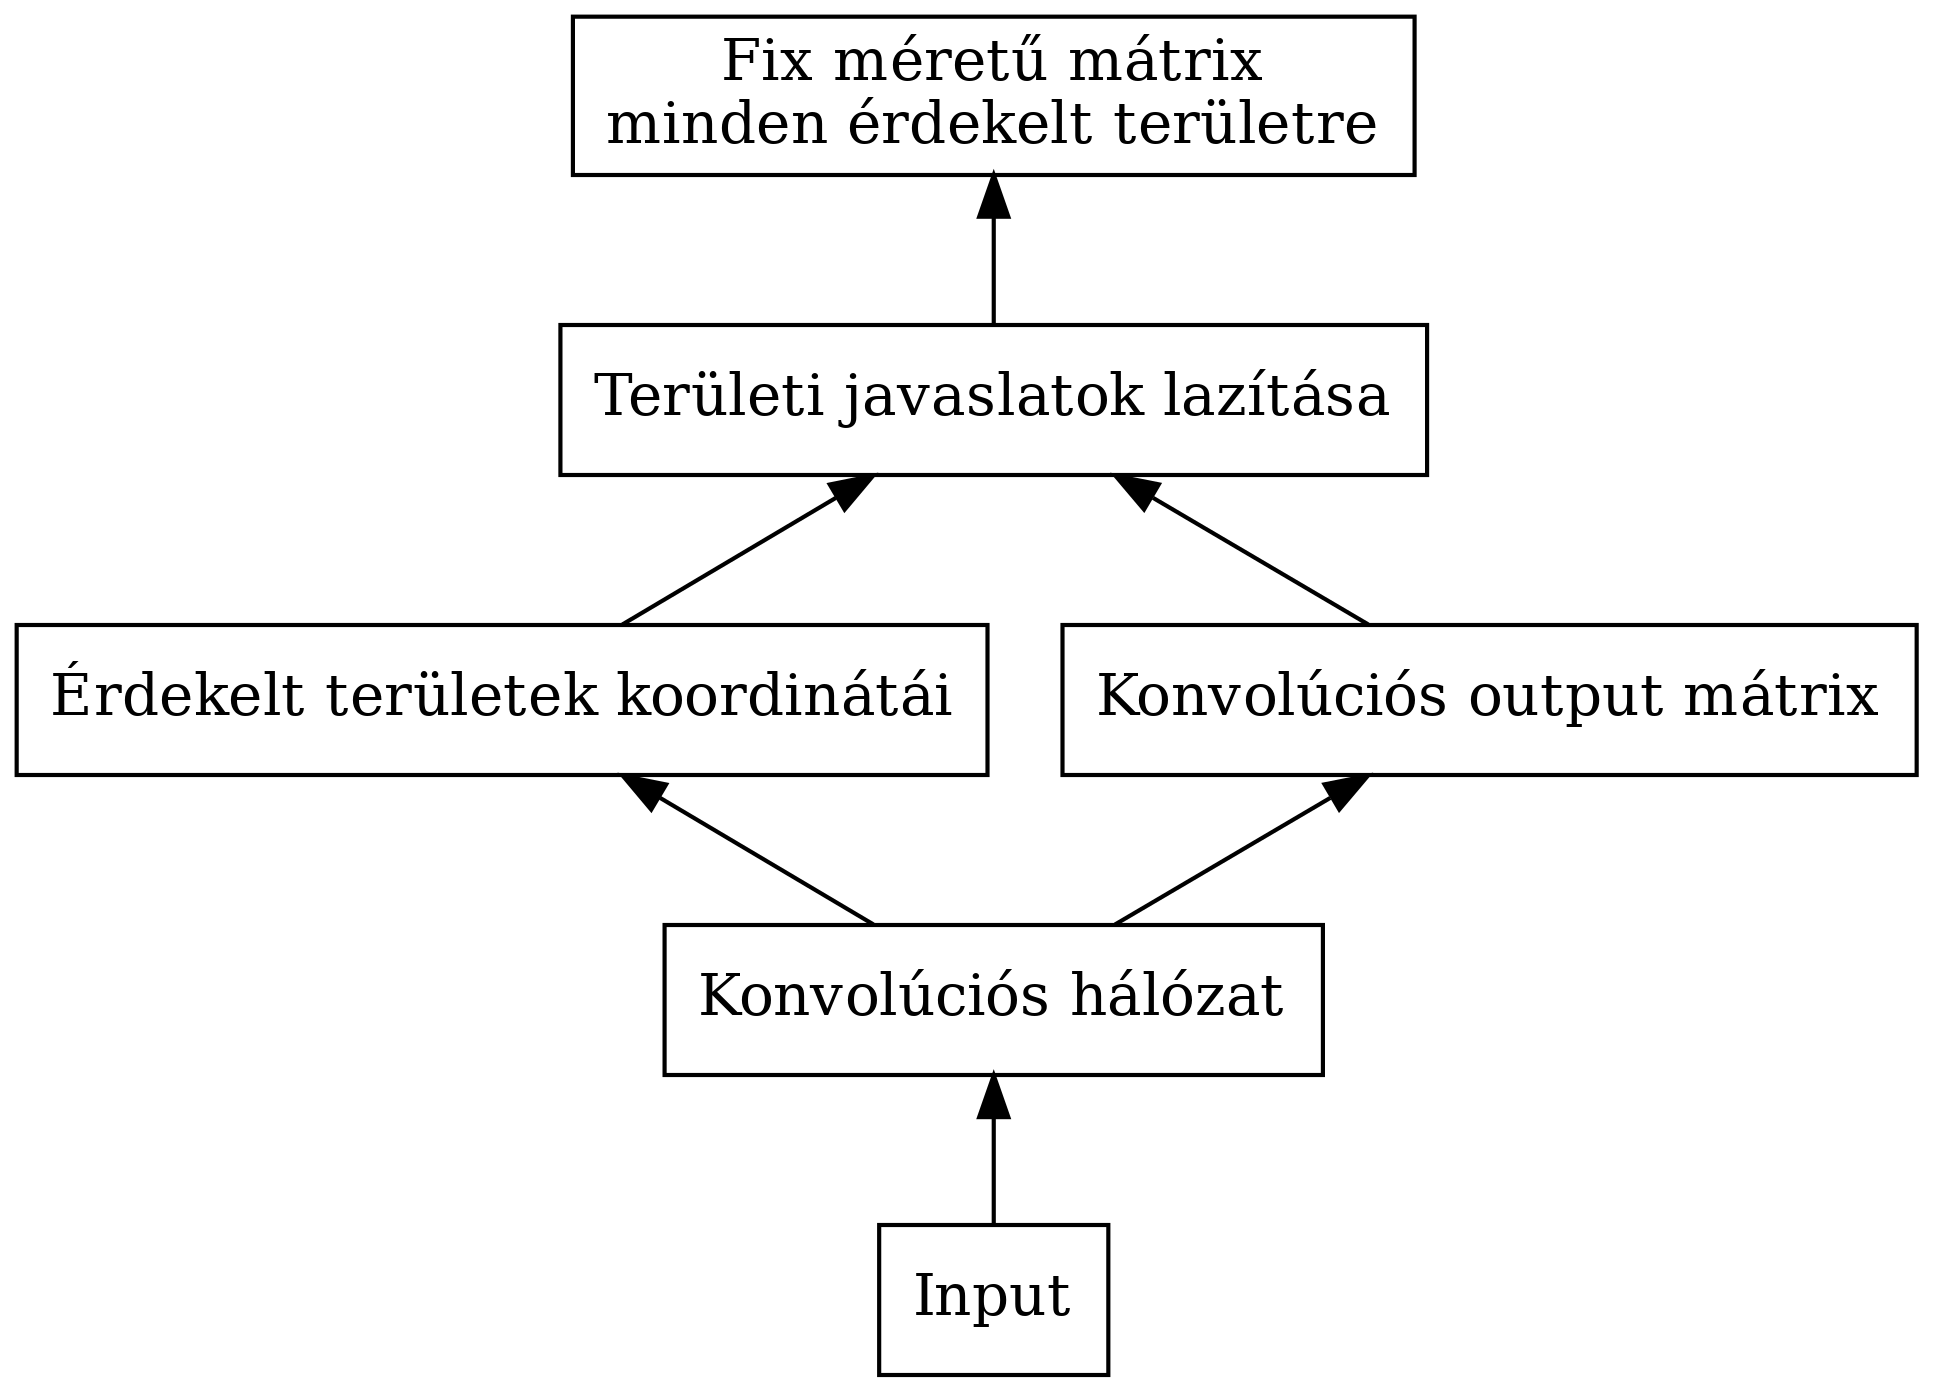
\includegraphics[height=7cm, width=7cm, keepaspectratio]{graphs/od_6.png}
\end{center}
\end{column}
\end{columns}
\end{frame}

\begin{frame}{Faster R-CNN}
\begin{columns}
\begin{column}{.5\textwidth}
A Faster R-CNN architektúra a \textbf{területi javaslatokat egy neurális hálózat segítségével} állítja elő (RPN).\par\smallskip
Ebben az esetben a területjavasoló hálózatnak már \textbf{tanítható súlyai} vannak. A teljes hálózatot 4 különböző költséggel tanítódik.\par\smallskip
A Faster R-CNN egy kétlépéses objektum detektor:
\begin{enumerate}
	\item \textbf{Első lépés}: Képenként egyszeri futtatással lefut a gerinc hálózat és a területjavasoló hálózat. 
	\item \textbf{Második lépés}: Régiónként egszeri futtatással 
\end{enumerate}
\end{column}
\begin{column}{.5\textwidth}
\begin{center}
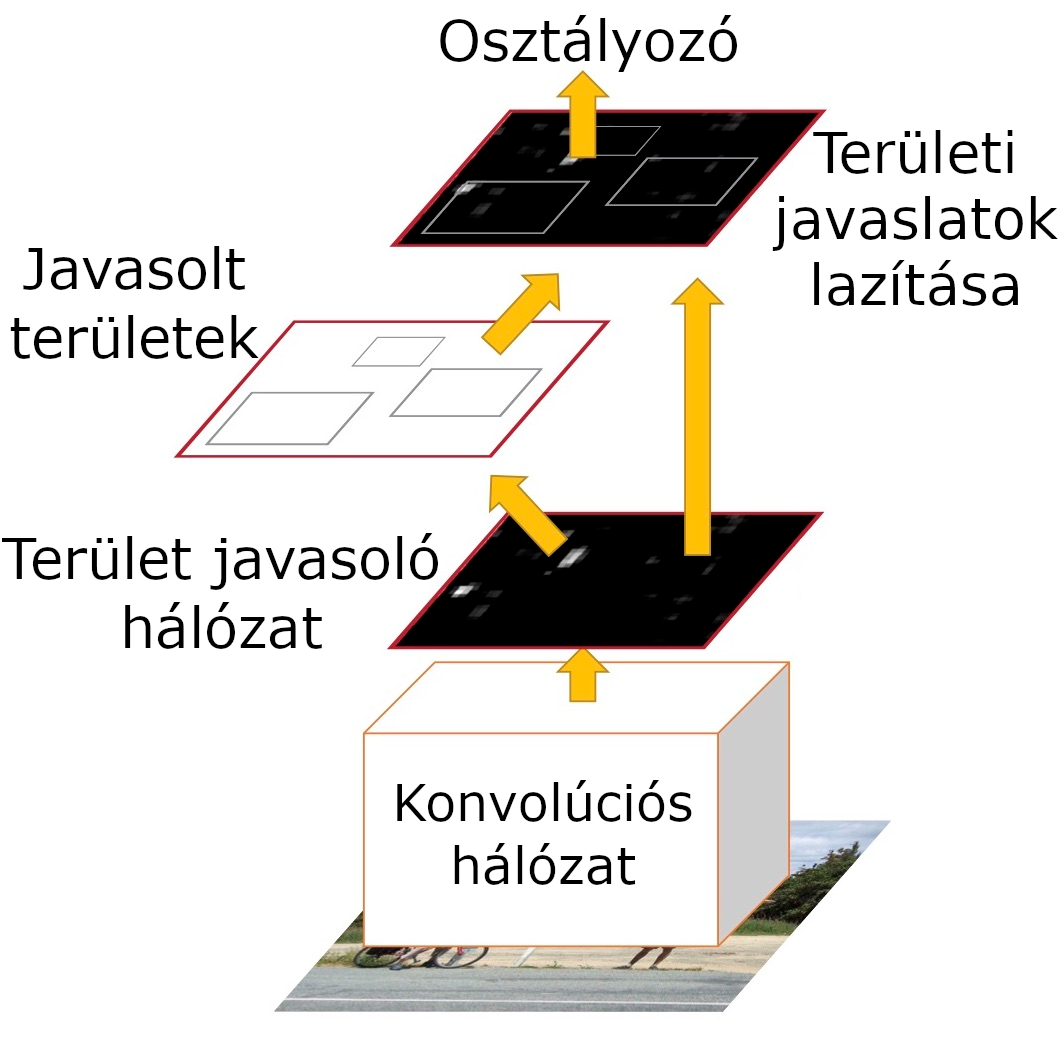
\includegraphics[width=6cm, height=7cm, keepaspectratio]{images/od_15.png}
\end{center}
\end{column}
\end{columns}
\end{frame}

\begin{frame}{Faster R-CNN}
\begin{columns}
\begin{column}{.5\textwidth}
\begin{enumerate}
	\item \textbf{RPN osztályozás}: A kereteződoboz objektum / nem objektum?
	\item \textbf{RPN regresszió}: A javasolt doboz és a kereteződoboz közötti transzformáció megbecslése.
	\item \textbf{Objektum osztáyozás}: A javaslatok osztályának megbecslése.
	\item \textbf{Objektum regresszió}: A javasolt doboz és objektum doboz közötti transzformáció megbecslése. 
\end{enumerate}
\end{column}
\begin{column}{.5\textwidth}
\begin{center}
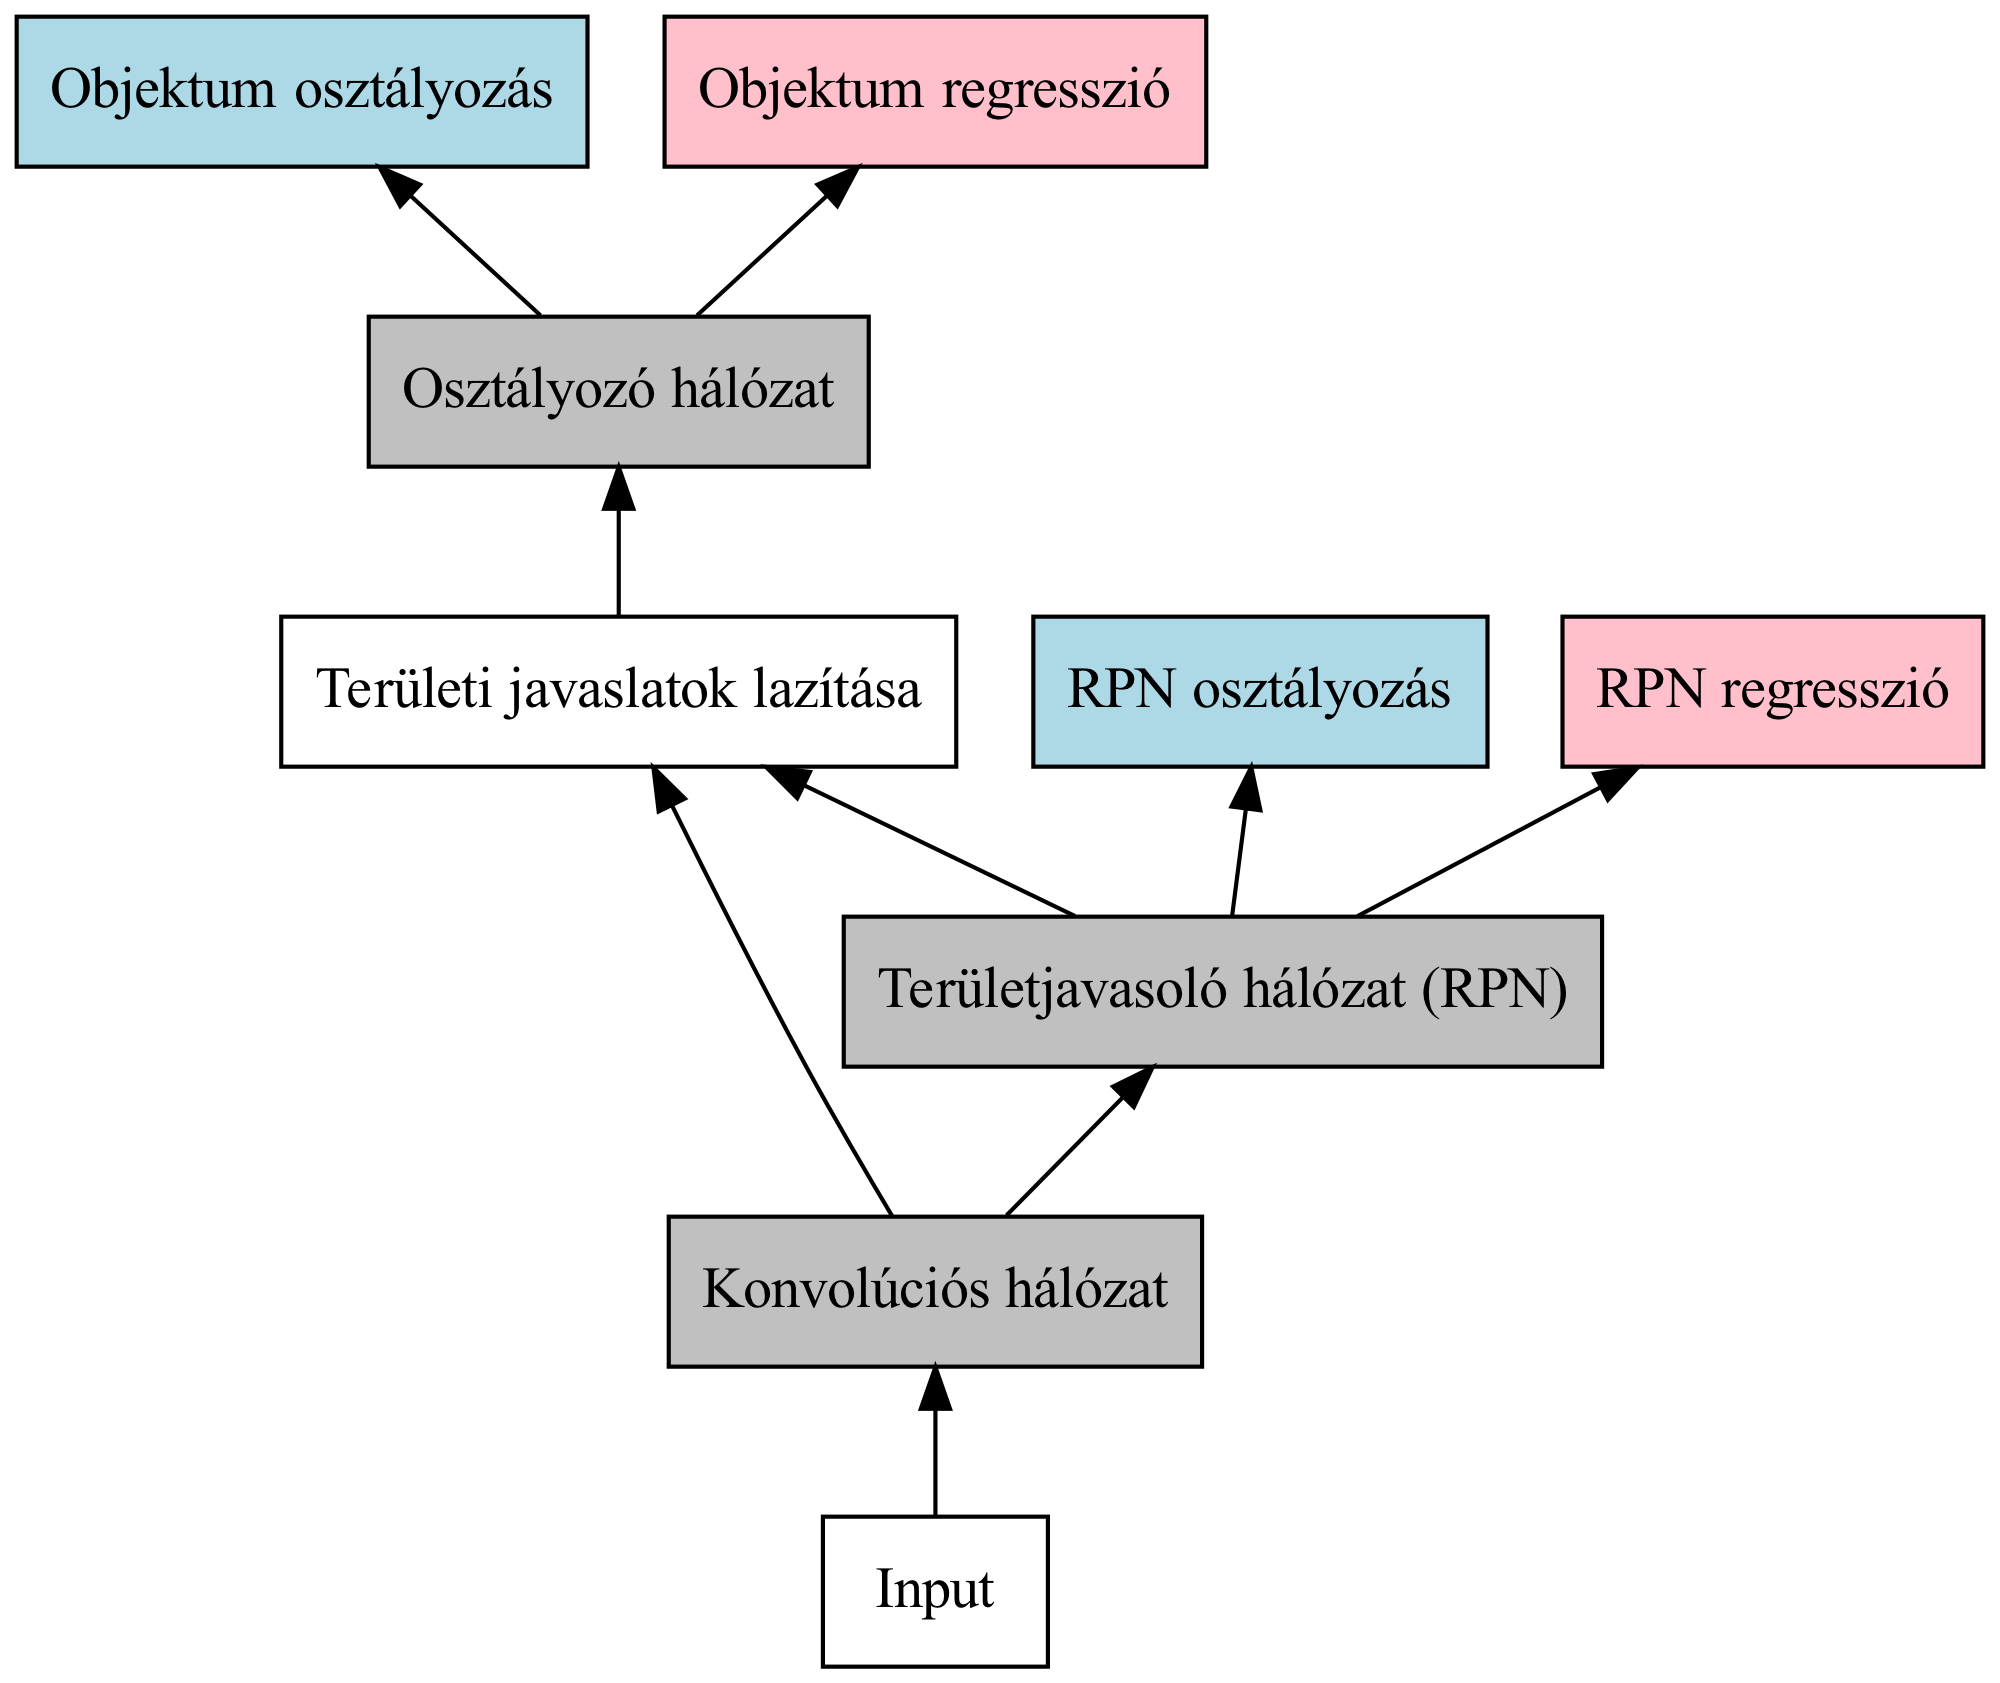
\includegraphics[width=7cm, height=7cm, keepaspectratio]{graphs/od_7.png}
\end{center}
\end{column}
\end{columns}
\end{frame}

\begin{frame}{Területjavasoló hálózat (RPN) - Osztályozás}
\only<1>{A területjavasoló hálózat minden képpont körül \textbf{egy rögzített méretű dobozt} hoz létre, amiről eldönti, hogy \textbf{objektum-e} (bináris osztályozás).}
\only<2>{Minden, az előző lépésben pozitívan osztályozott kereteződobozra a területjavasoló hálózat egy \textbf{korrekciót generál}, ami \textbf{módosíthat az eredeti kereteződoboz} koordinátáin, hogy jobban illeszkedjen a dobozban megtalálható objektumra.}
\only<1>{\begin{center}
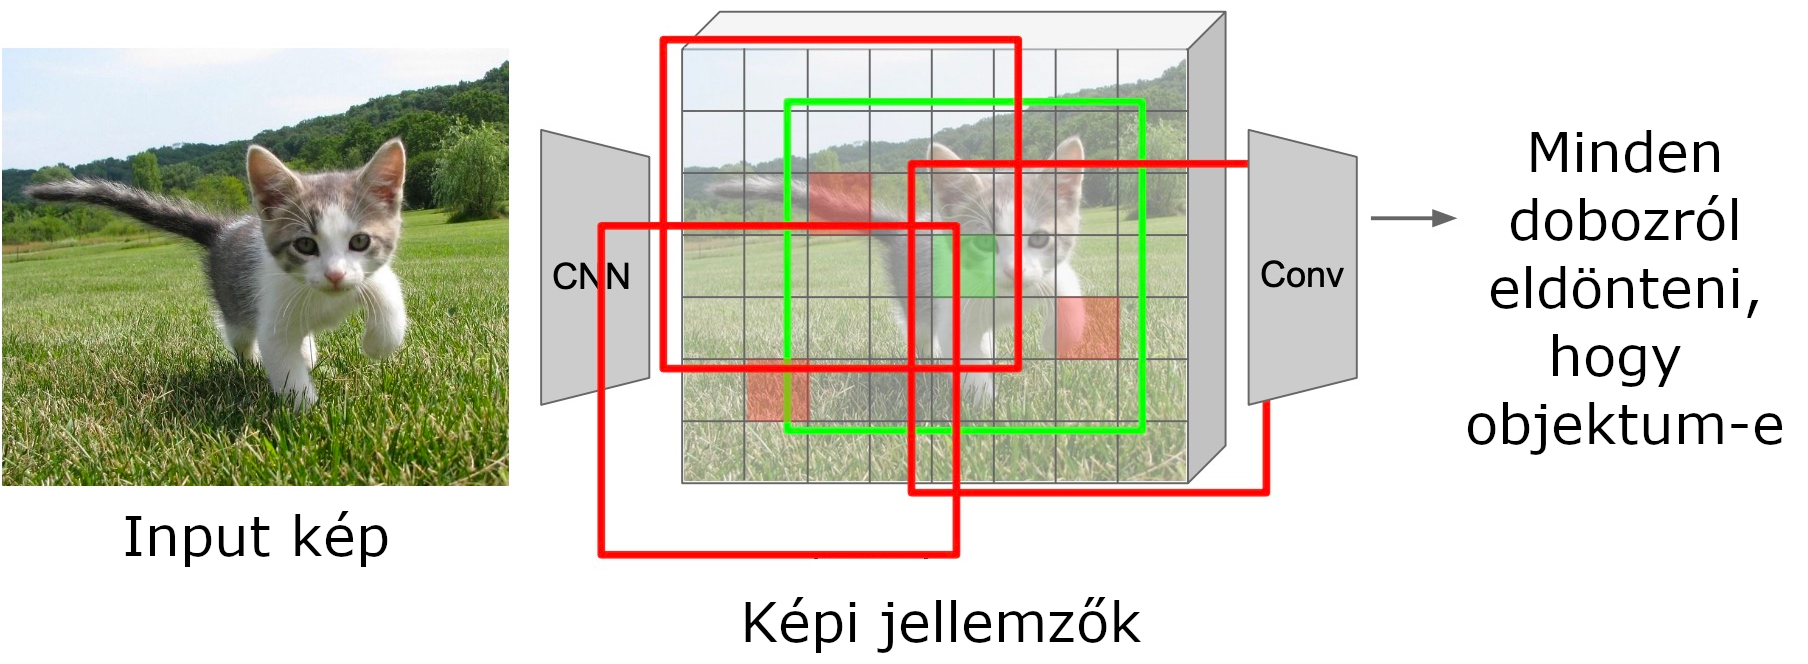
\includegraphics[width=12cm, keepaspectratio]{images/od_16.png}
\end{center}}
\only<2>{\begin{center}
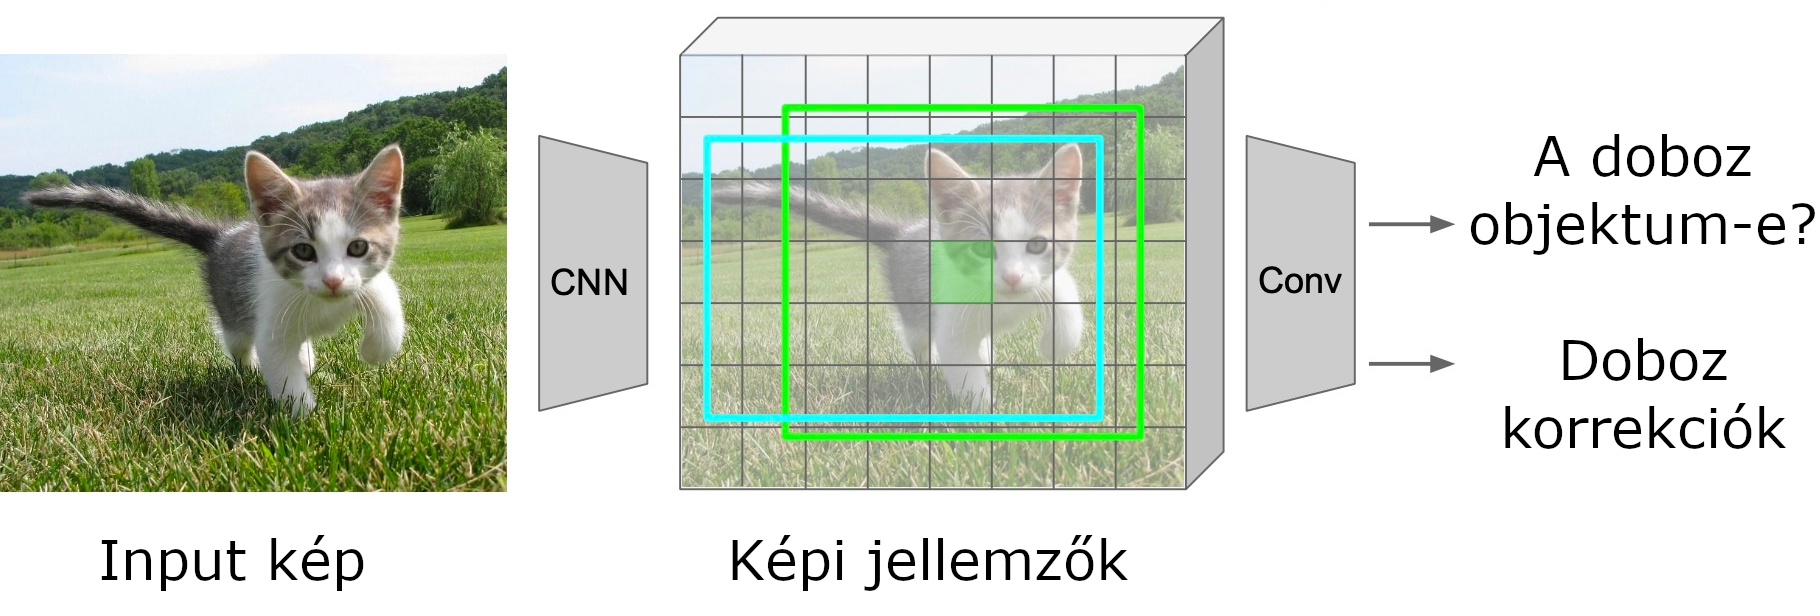
\includegraphics[width=12cm, keepaspectratio]{images/od_17.png}
\end{center}}
\end{frame}

\begin{frame}{Egylépéses detekció - YOLO architektúra}
\begin{columns}
\begin{column}{.5\textwidth}
A YOLO (You Only Look Once) architektúra egy népszerű objektum detektor konfiguráció.\par\smallskip
Ebben az esetben a hálózat az input képet \textbf{felosztja egy $n \cdot n$ db cellából álló hálóra}. Minden cellához hozzárendel $B$ db \textbf{alapdobozt}, amelynek középpontja a cella közepe.\par\smallskip
Minden cellára a hálóban megbecsül a $B$ db alapdobozból 5 értéket: $[dx, dy, dh, dw, p]$ ahol az első $4$ érték az eltolást jelenti $x, y, w, h$ dimenziók mentén, $p$ pedig a softmax aktiváció minden osztályra, beleértve a hátteret is. 
\end{column}
\begin{column}{.5\textwidth}
\begin{center}
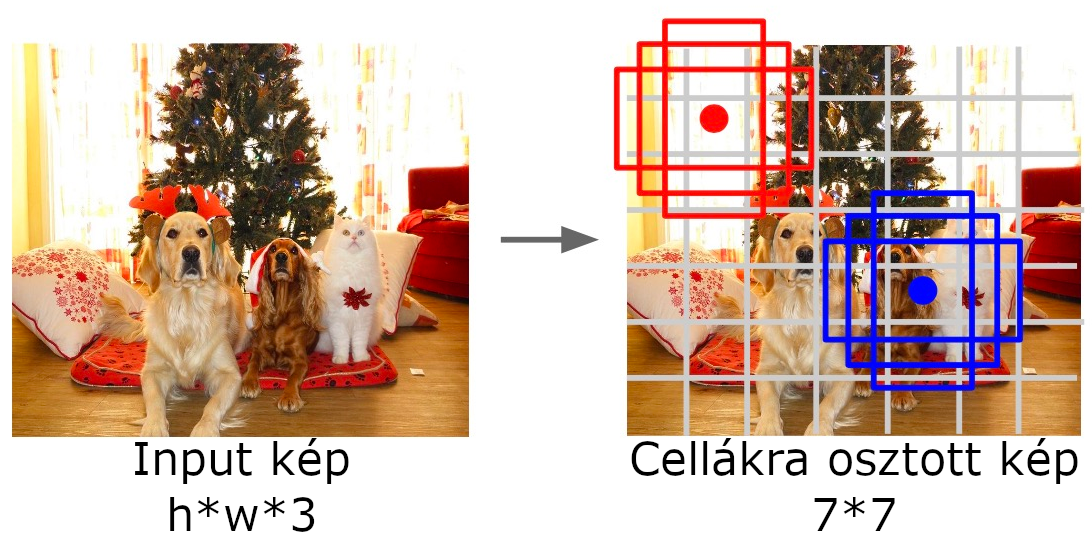
\includegraphics[width=7cm, keepaspectratio]{images/od_19.png}
\end{center}
A YOLO hálózat outputja ebben az esetben $7 \cdot 7 \cdot (5 \cdot B + C)$, ahol $C$ a lehetséges osztályok száma.
\end{column}
\end{columns}
\end{frame}

\end{document}














